\documentclass[11pt,a4paper]{article}

% ======================================================================
%  16C(d,p)17C analysis report -- full internal/collaboration writeup
%  Self-contained: compiles on Overleaf (pdfLaTeX + BibTeX) as-is.
% ======================================================================

\usepackage[utf8]{inputenc}
\usepackage[T1]{fontenc}
\usepackage{amsmath,amssymb}
\usepackage{graphicx}
\usepackage{booktabs}
\usepackage{siunitx}
\usepackage[margin=2.4cm]{geometry}
\usepackage{xcolor}
\usepackage{caption}
\usepackage{subcaption}
\usepackage[hidelinks]{hyperref}
\usepackage{microtype}

\graphicspath{{figs/}}
\captionsetup{font=small,labelfont=bf}

\newcommand{\Cs}{$^{16}$C}
\newcommand{\Cse}{$^{17}$C}
\newcommand{\dp}{(d,p)}
\newcommand{\dsdo}{$\mathrm{d}\sigma/\mathrm{d}\Omega$}
\newcommand{\chinu}{$\chi^2/\nu$}
\newcommand{\thcm}{$\theta_{\mathrm{c.m.}}$}
\newcommand{\Ex}{$E_x$}
\newcommand{\mevu}{\,MeV/u}

% editorial flag
\newcommand{\note}[1]{\textcolor{red!70!black}{[#1]}}

\title{\textbf{Spectroscopy of unbound \Cse\ states via the \Cs\dp\Cse\
reaction at FRIB (experiment a1975)}\\[2pt]
\large Angular distributions, absolute normalization, and $L$ assignments}
\author{Y.~Ayyad\\
\small IGFAE, Universidade de Santiago de Compostela}
\date{\today}

\begin{document}
\maketitle

\begin{abstract}
\noindent
We report the extraction of absolute differential cross sections
($\mathrm{d}\sigma/\mathrm{d}\Omega$) for states of \Cse\ populated in the
\Cs\dp\Cse\ transfer reaction at $11.77$\mevu, measured with the AT-TPC at
FRIB (experiment a1975). Three bound states and seven unbound resonances are
isolated through an angle-binned spectral fit of the $Q$-corrected excitation
energy. The absolute scale is fixed by a self-contained optical-model analysis
of the \Cs$(d,d)$ elastic channel, which shares the entrance partition with the
transfer; the residual normalization uncertainty is $\sim$12\,\% (the spread
across optical potentials), carried as a correlated global scale. Orbital
angular momenta are assigned by comparing each angular distribution to FRESCO
ADWA single-particle shapes. A localized excess near $E_x\simeq0.45$~MeV, which
concentrates at backward angles, is documented and carried as a model-dependence
systematic. Results are compared to the previous in-house \Cs\dp\ analysis of
Movilla and Ayyad, and the bound-state spectroscopic factors are benchmarked
against the published measurement of Pereira-Lopez \textit{et al.} (PLB 811,
135939), which they reproduce within $\sim$$1\sigma$ for the $1/2^+$ and $5/2^+$
states. The effective spectroscopic factors for the unbound resonances are
shape-only (the weakly-bound approximation gives the correct angular shape but
an artificial magnitude) and a continuum treatment is required for
publication-grade values.
\end{abstract}

\tableofcontents

% ======================================================================
\section{Introduction and motivation}
\label{sec:intro}

The neutron-rich carbon isotope \Cse\ sits near the $N=14$ subshell and its
single-particle structure probes the evolution of the $sd$ shell far from
stability. Bound-state spectroscopy and the lowest unbound resonances have been
studied previously in \Cs\dp\ transfer~\cite{PereiraLopez2020,MovillaAyyad2026};
the present work extends that program to the full set of seven unbound
resonances accessible in experiment a1975, with an emphasis on (i) placing the
angular distributions on an \emph{absolute} cross-section scale, (ii) a
controlled treatment of the non-resonant continuum and a near-threshold
contaminant, and (iii) transferred-$L$ assignments with quantified systematic
uncertainties.

This document is an internal analysis report: it records the method, the data
products, every cut and correction, and the open items, at a level of detail
sufficient to reproduce the numbers. Editorial placeholders are marked in
\note{red}.

% ======================================================================
\section{Reaction and experimental setup}
\label{sec:exp}

A \Cs\ beam at a total energy of $188.33$~MeV ($11.77$\mevu;
$Q_{\mathrm{g.s.}}=-1.498$~MeV) impinged on the deuterated active gas of the
AT-TPC~\cite{Bradt2017}, which served simultaneously as the D$_2$ target and the
tracking detector. Recoil protons from \Cs\dp\Cse\ were reconstructed
event-by-event; the magnetic rigidity, polar and azimuthal angles, and the
reaction vertex are provided by the ATTPCROOT \texttt{InterpSolver} reduction
(tree \texttt{parquettree}). The proton energy is obtained from the rigidity,
\begin{equation}
  p_{\mathrm{ej}} = B\rho\,z_{\mathrm{ej}}\,c,
  \qquad
  E_{\mathrm{ej}} = \sqrt{p_{\mathrm{ej}}^2 + m_p^2} - m_p ,
\end{equation}
and the excitation energy $E_x$ and centre-of-mass angle \thcm\ follow from
relativistic two-body kinematics. A per-event, vertex-dependent $Q$-correction
is applied,
$E_x^{\rm corr} = E_x^{\rm raw} - p_1 z - p_0 + \mathrm{offset} + \Delta_Q$,
with the constants inherited from the parent analysis.

The seven unbound resonances and their literature assignments are listed in
Table~\ref{tab:states}. The analysis uses 47 runs and the nominal event
selection (polar angle $\ge 90^\circ$); a ``strict'' selection
($E_{\mathrm{ej}}<8$~MeV and vertex $z\in[2,98]$~cm) is used as a systematic.

\begin{table}[t]
  \centering
  \caption{Unbound \Cse\ resonances included in the spectral fit, with the
  literature $J^\pi$ and the initial resonance width $\Gamma$ used to seed the
  penetrability-modified Breit--Wigner lineshape.}
  \label{tab:states}
  \begin{tabular}{ccc}
    \toprule
    $E_x$ (MeV) & $J^\pi$ & $\Gamma$ (keV) \\
    \midrule
    2.763 & $1/2^-$        & 50  \\
    2.980 & $3/2^+$        & 200 \\
    3.661 & \emph{new}     & 398 \\
    4.231 & $3/2^+$        & 500 \\
    4.841 & $1/2^+$        & 300 \\
    5.91  & $3/2^+$        & 1500\\
    6.30  & $5/2^+$        & 396 \\
    \bottomrule
  \end{tabular}
\end{table}

% ======================================================================
\section{Spectral fitting}
\label{sec:spectral}

\subsection{Model}
The $Q$-corrected $E_x$ spectrum is fitted with a composite model:
three Gaussians for the bound states; seven penetrability-modified
Breit--Wigner (BW) lineshapes for the unbound resonances; one-neutron and
two-neutron phase-space templates (simulated, loaded per angular bin); and a
linear background. The BW lineshape uses an energy-dependent width via tabulated
$n+$\Cs\ penetrabilities for $L=0$--3 and an analytic Voigt convolution with the
experimental resolution,
\begin{equation}
  \mathrm{BW}(E) = A\cdot 2\pi\,\mathrm{Voigt}\!\big(E-E_0,\ \sigma,\
  \Gamma_{\rm eff}(E)\big),
  \qquad
  \Gamma_{\rm eff}(E)=\Gamma_0\,\frac{T_L(E)}{T_L(E_0)} ,
\end{equation}
which is $\sim$$10^3\times$ faster than the numerical convolution used in the
original macro and exact in the constant-$\Gamma$-per-step limit.

\subsection{Angle-binned procedure}
The spectrum is binned in \thcm\ in $12\times2.5^\circ$ bins over
$10$--$40^\circ$, plus an inclusive $10$--$40^\circ$ histogram. An
\emph{inclusive} fit first fixes the resonance positions, widths, and
resolution. Each angular bin is then refitted with positions and widths frozen
and only the amplitudes free (Gaussians, BWs, both phase-space terms, and the
linear background). The inclusive and per-bin fits are shown in
Figs.~\ref{fig:inclusive} and~\ref{fig:perbin}. Integrated yields and
$\mathrm{d}\sigma/\mathrm{d}\Omega$ are written per state per bin.

\begin{figure}[t]
  \centering
  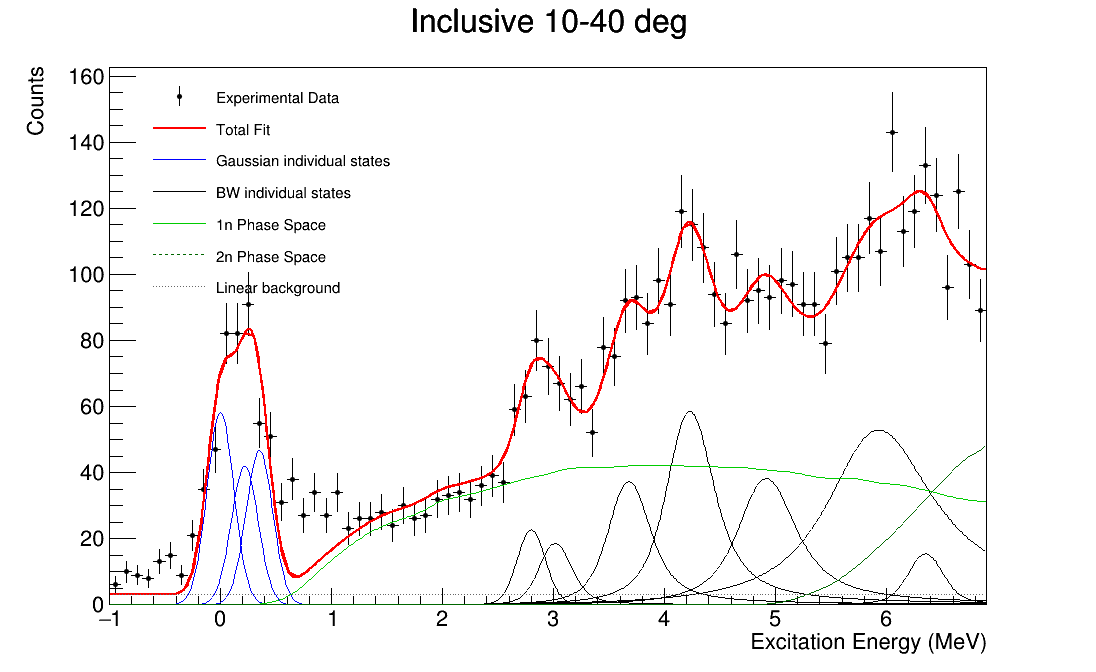
\includegraphics[width=0.78\linewidth]{plots_inclusive.png}
  \caption{Inclusive $Q$-corrected $E_x$ spectrum (\thcm\ $=10$--$40^\circ$)
  with the composite fit: bound-state Gaussians, penetrability-modified
  Breit--Wigners, 1n/2n phase space, and linear background.}
  \label{fig:inclusive}
\end{figure}

\begin{figure}[t]
  \centering
  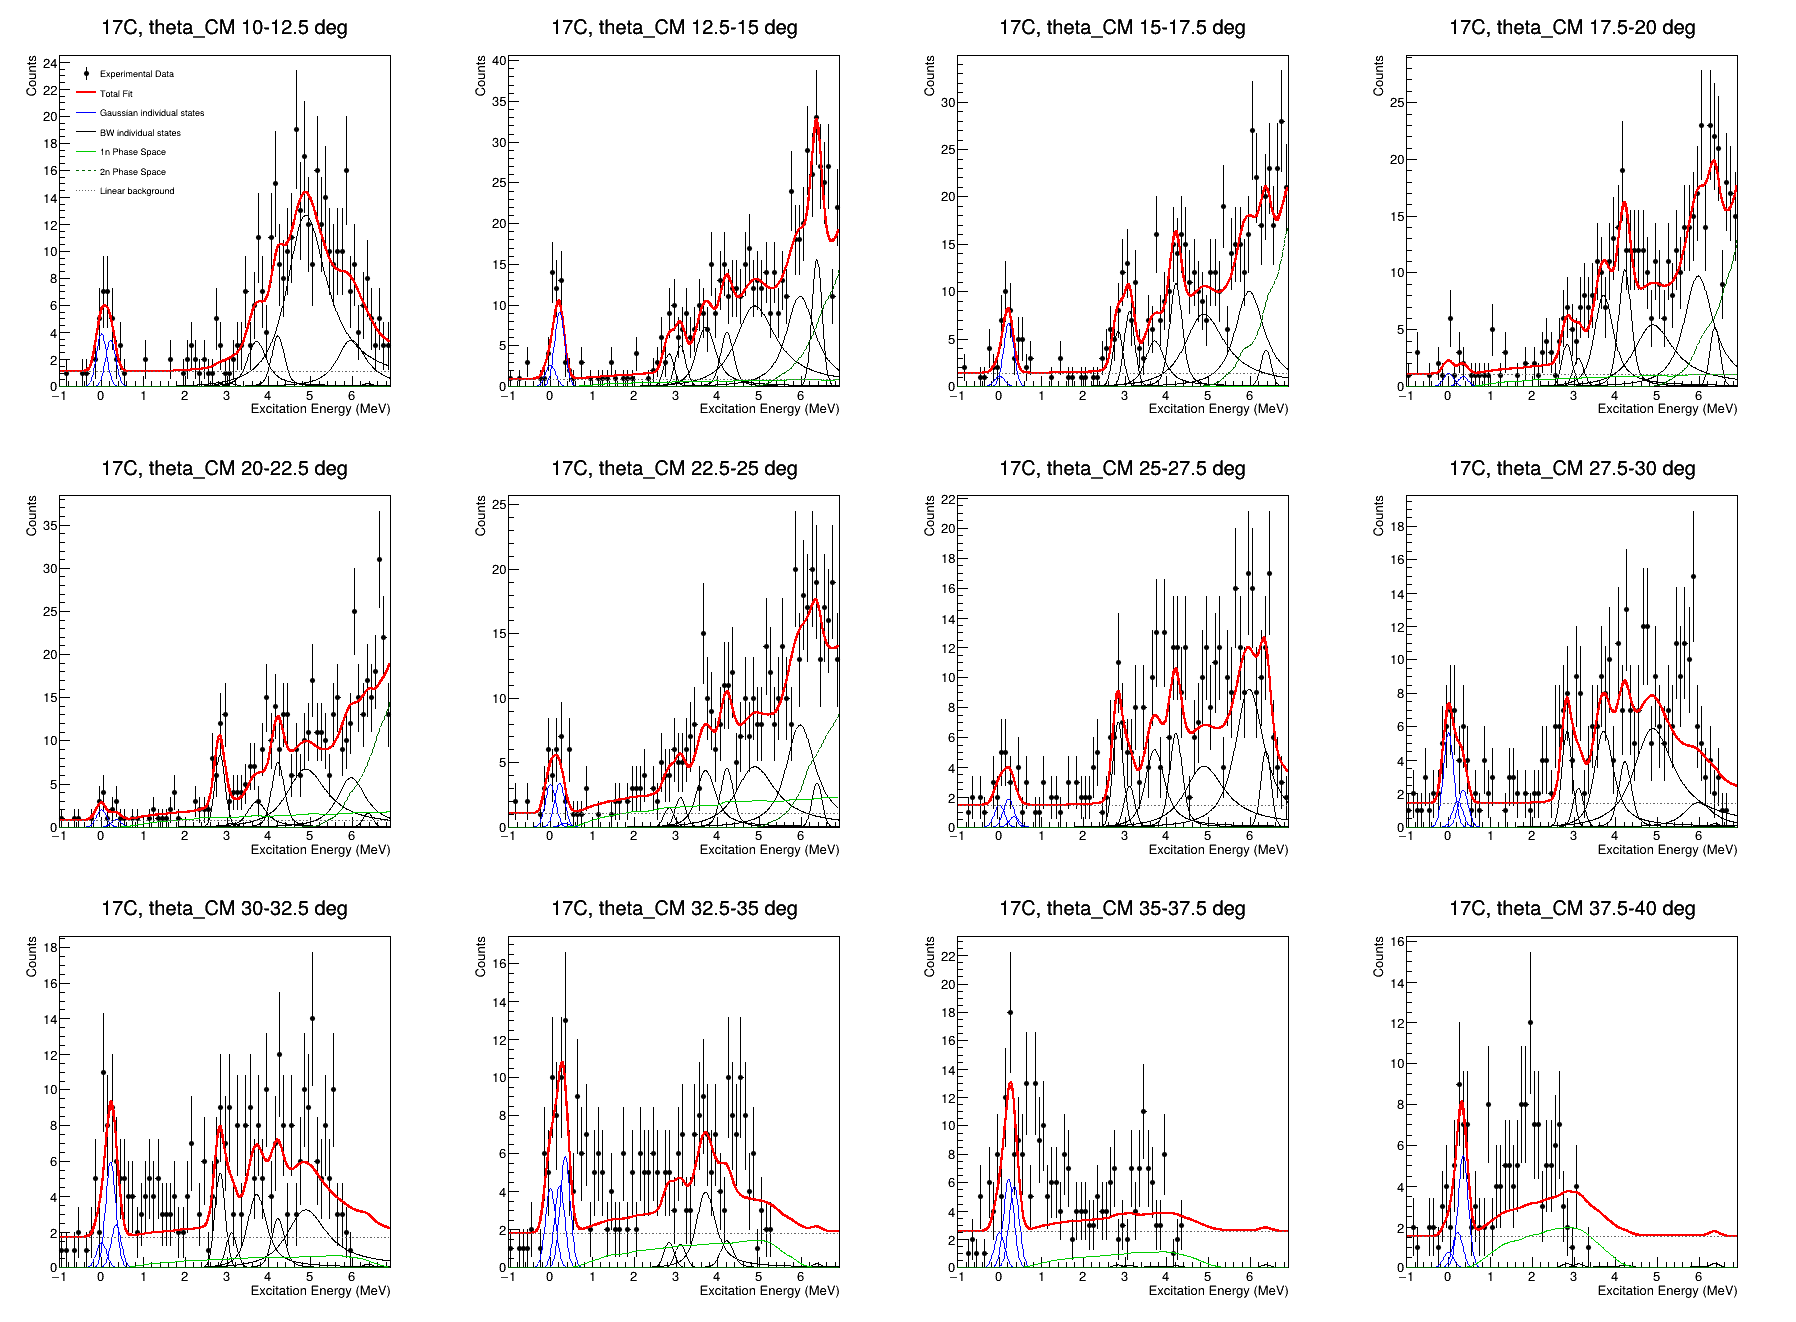
\includegraphics[width=\linewidth]{per_bin_fits.png}
  \caption{Per-angular-bin fits ($2.5^\circ$ bins, $10$--$40^\circ$). Resonance
  positions and widths are frozen from the inclusive fit; only amplitudes vary.
  Forward bins are resonance-dominated; beyond $\sim$$30^\circ$ the transfer
  peaks fade and the continuum dominates the shape.}
  \label{fig:perbin}
\end{figure}

\subsection{The near-threshold contaminant}
\label{sec:contam}
The inclusive residuals reveal a localized $+2$--$4\sigma$ excess at
$E_x\simeq0.4$--$1.1$~MeV that the nominal model cannot absorb
(Fig.~\ref{fig:residuals}). Adding a fourth Gaussian whose centroid pegs at
$\simeq0.45$~MeV restores an acceptable fit; the inclusive \chinu\ drops as
summarized in Table~\ref{tab:chi2grid}. The excess survives the strict event
selection (centroid $0.450\!\to\!0.451$~MeV), so it is not an AT-TPC
edge/track artifact. It is therefore carried as a model-dependence systematic
rather than removed. Its physical nature is examined in
Sec.~\ref{sec:contam-fingerprint}.

\begin{table}[h]
  \centering
  \caption{Inclusive-fit \chinu\ for the four combinations of event selection
  (loose/strict) and contaminant Gaussian (off/on).}
  \label{tab:chi2grid}
  \begin{tabular}{lcc}
    \toprule
    cuts $\backslash$ contaminant & nominal & $+$ contam.\ Gauss \\
    \midrule
    loose  & 1.78 & \textbf{0.84} \\
    strict & 1.88 & \textbf{0.97} \\
    \bottomrule
  \end{tabular}
\end{table}

\begin{figure}[t]
  \centering
  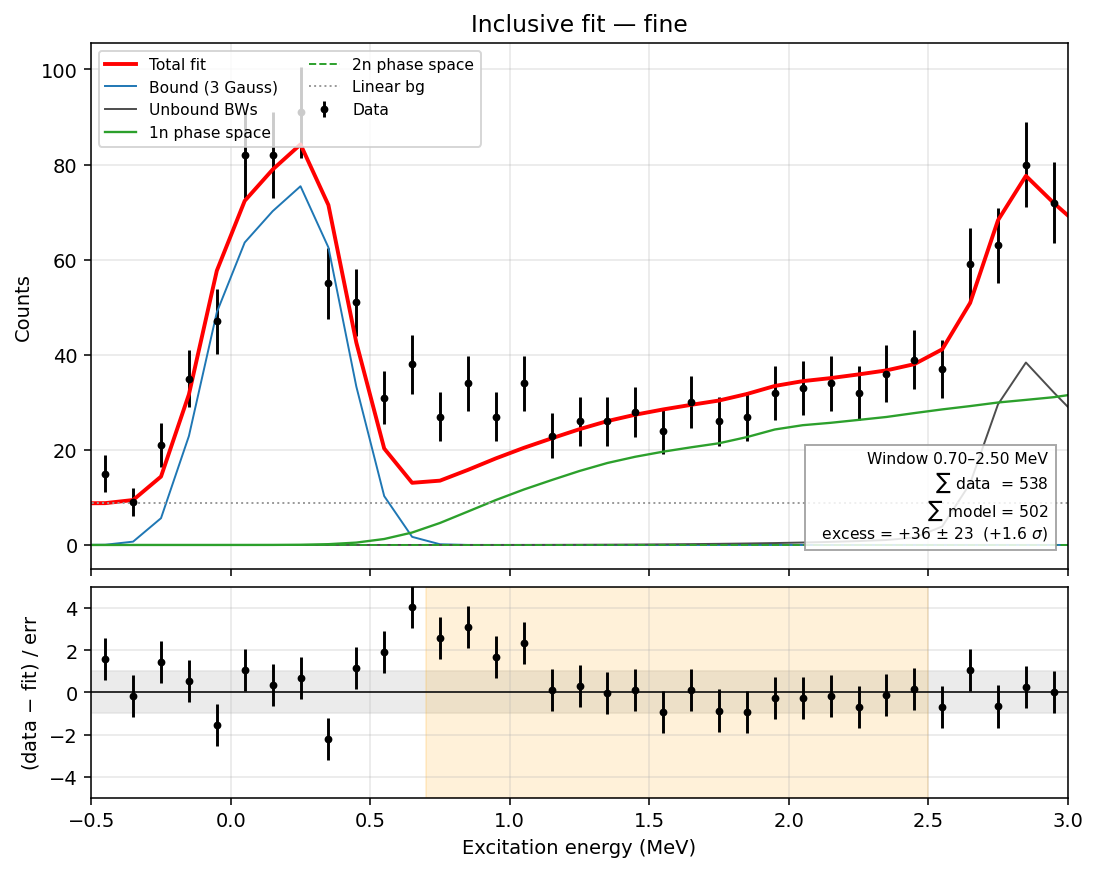
\includegraphics[width=0.72\linewidth]{inclusive_residuals_fine.png}
  \caption{Inclusive-fit residuals in the $0$--$3$~MeV region, showing the
  localized excess near $0.45$--$1.1$~MeV that motivates the contaminant
  Gaussian.}
  \label{fig:residuals}
\end{figure}

% ======================================================================
\section{Bound states}
\label{sec:bound}

The three bound states---the ground state ($3/2^+$), the $0.217$~MeV ($1/2^+$),
and the $0.335$~MeV ($5/2^+$)---are extracted primarily as a cross-check of the
machinery (efficiency correction and absolute scale) before the unbound region.
Their angular distributions are shown together in Fig.~\ref{fig:bound}. The
ground state and $0.217$~MeV state are forward-peaked and consistent with their
expected $\ell$ content; the $5/2^+$ at $0.335$~MeV is only weakly populated and
its points sit near the detection floor (shown for completeness). The
$35$--$40^\circ$ bins reach the fit floor at the AT-TPC kinematic edge and are
excluded for the bound states.

\begin{figure}[t]
  \centering
  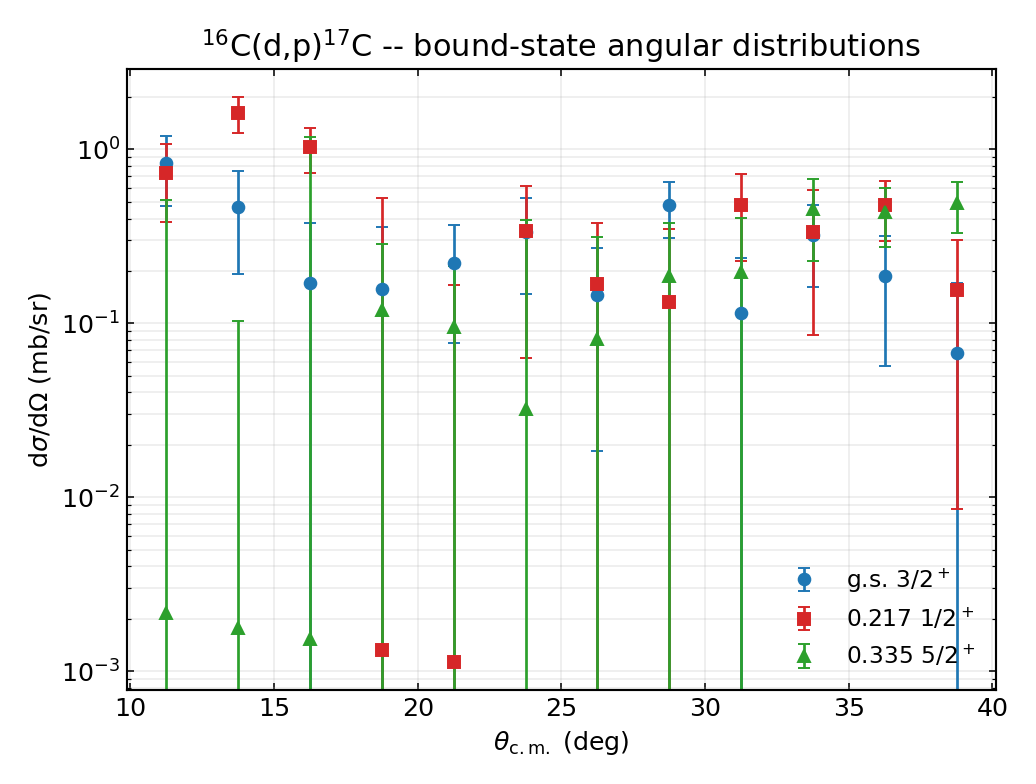
\includegraphics[width=0.7\linewidth]{bound_states_ad.png}
  \caption{Angular distributions of the three bound \Cse\ states (this work,
  $2.5^\circ$ binning, corrected statistical errors).}
  \label{fig:bound}
\end{figure}

% ======================================================================
\section{Absolute normalization}
\label{sec:norm}

\subsection{Method}
Counts are converted to a differential cross section via a fixed luminosity
constant,
\begin{equation}
  \frac{\mathrm{d}\sigma}{\mathrm{d}\Omega}(\theta)
  = \frac{Y}{N_{\rm beam}\,N_{\rm target}\,\Delta\Omega}\cdot 10\ \Big/\
    \varepsilon ,
  \qquad
  \Delta\Omega = 2\pi(\cos\theta_{\rm lo}-\cos\theta_{\rm hi}),
\end{equation}
with $N_{\rm beam}=1.6146\times10^{5}$ and $N_{\rm target}=0.019632$ (the
calibrated beam$\times$target product inherited from the bound-state work), the
factor 10 converting fm$^2\!\to$mb, and $\varepsilon$ the detection efficiency
(Sec.~\ref{sec:eff}). The conversion was verified arithmetically: the
ground-state $10$--$12.5^\circ$ point reproduces from the yields table
($Y=11.55\Rightarrow\mathrm{d}\sigma/\mathrm{d}\Omega=0.829$~mb/sr).

\subsection{Validation against \Cs$(d,d)$ elastic}
The elastic channel shares the entrance partition---same beam, D$_2$ target,
and luminosity---so an absolute optical-model (OM) elastic cross section that
reproduces the measured \Cs$(d,d)$ angular distribution fixes the
$(N_{\rm beam}\,N_{\rm target})$ constant with no free normalization. A
self-contained partial-wave solver (Numerov integration with matching to
Coulomb functions; verified against Rutherford in the point-charge limit to
$10^{-3}$) was written for this purpose. At $E_{\rm lab}(d)=23.55$~MeV
($E_{\rm c.m.}=20.92$~MeV) the forward-lobe error-weighted ratio
$\langle\mathrm{data}/\mathrm{OM}\rangle$ is reported for three potentials in
Table~\ref{tab:omp} and Fig.~\ref{fig:elastic}.

\begin{table}[h]
  \centering
  \caption{Forward-lobe $\langle$data/OM$\rangle$ for the \Cs$(d,d)$ elastic
  channel and three optical potentials (re-run 2026-05-30).}
  \label{tab:omp}
  \begin{tabular}{lcc}
    \toprule
    optical potential & \chinu & $\langle$data/OM$\rangle$ \\
    \midrule
    ADWA (transfer OMP)         & 398 & 0.864 \\
    DA1p (light-target global)  & 105 & 0.886 \\
    free 5-parameter fit        & 32  & \textbf{0.978} \\
    \bottomrule
  \end{tabular}
\end{table}

\begin{figure}[t]
  \centering
  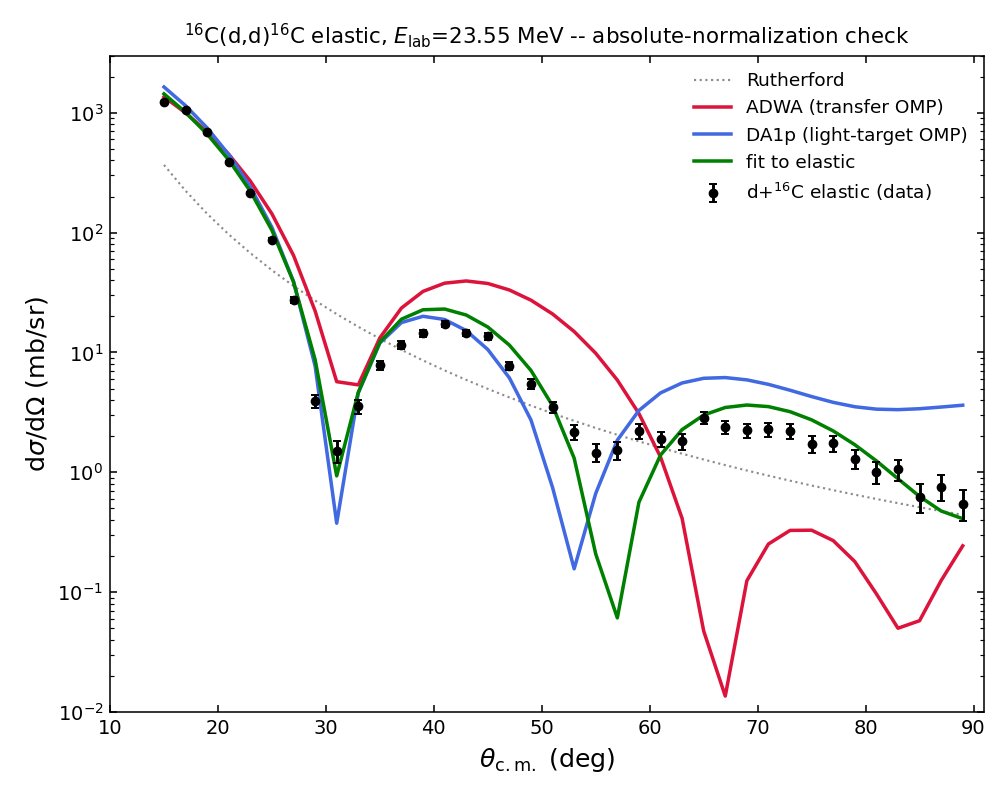
\includegraphics[width=0.66\linewidth]{om_elastic_dd.png}
  \caption{\Cs$(d,d)$ elastic angular distribution (data) versus three optical
  potentials. The absolute scale is robust in the forward Coulomb--nuclear
  lobe.}
  \label{fig:elastic}
\end{figure}

The free-fit potential reproduces the absolute scale to $\sim$2\,\%
($0.978\pm0.043$); however, the ADWA potential actually used in the transfer
DWBA sits $\sim$14\,\% below the data. The honest normalization uncertainty is
therefore the \emph{cross-potential spread}, $\approx0.86$--$0.98$
($\sim$12\,\%). This is a global, fully correlated scale that shifts all states
and angles together; it is \emph{not} folded into the per-point error but
quoted separately and provided as outer bands in
\texttt{results/\{dsdo,yield\}\_bands\_fine.csv}.

\subsection{Efficiency correction}
\label{sec:eff}
Detection efficiency in the AT-TPC depends on the proton energy (hence $E_x$)
as well as $\theta$. Eight simulated tables at $E_x=0,2,3,4,4.8,5,5.9,6$~MeV,
each $5^\circ$-spaced in $\theta$, are interpolated bilinearly in
$(E_x,\theta)$; the three bound states use the $E_x=0$ table. Two protections
are applied per (state, bin): an $\varepsilon$-floor cut (drop bins with
$\varepsilon<0.15$, where the correction blows up) and an $\varepsilon$-gradient
cut (drop bins where $\varepsilon$ varies by more than a factor 2 across the bin
width, so a bin-centre value is meaningless).

\subsection{Per-point error model}
The per-point statistical error is
\begin{equation}
  \delta\!\left(\frac{\mathrm{d}\sigma}{\mathrm{d}\Omega}\right)
  = \frac{\mathrm{d}\sigma}{\mathrm{d}\Omega}
    \sqrt{\left(\frac{\delta Y}{Y}\right)^2
        + \left(\frac{\delta\varepsilon}{\varepsilon}\right)^2 },
\end{equation}
where $\delta Y$ is the Minuit amplitude error from the per-bin $\chi^2$ fit to
$\sqrt{N}$-weighted histograms and therefore already carries the Poisson
statistics of the yield. A previous version added a redundant $1/Y$ Poisson term
($\sqrt{1/Y+(\delta Y/Y)^2}$), double-counting the statistics ($\sqrt{2}$
inflation in the Poisson-dominated limit); this was corrected (e.g.\ the
ground-state $10$--$12.5^\circ$ error went $0.433\to0.356$~mb/sr). Three
uncertainty layers are kept distinct throughout: \emph{statistical} (per point),
\emph{systematic} (the 82-variant envelope, Sec.~\ref{sec:syst}), and the
\emph{global scale} ($\sim$12\,\%, above).

% ======================================================================
\section{Angular distributions and \texorpdfstring{$L$}{L} assignments}
\label{sec:Lassign}

\subsection{Extracted distributions}
The absolute \dsdo\ for the seven unbound resonances are shown in
Fig.~\ref{fig:adgrid}, each with the per-point statistical error and the
82-variant systematic band. Fits to FRESCO shapes use only \thcm\ $\le30^\circ$,
where the resonance signal dominates over the continuum.

\begin{figure}[t]
  \centering
  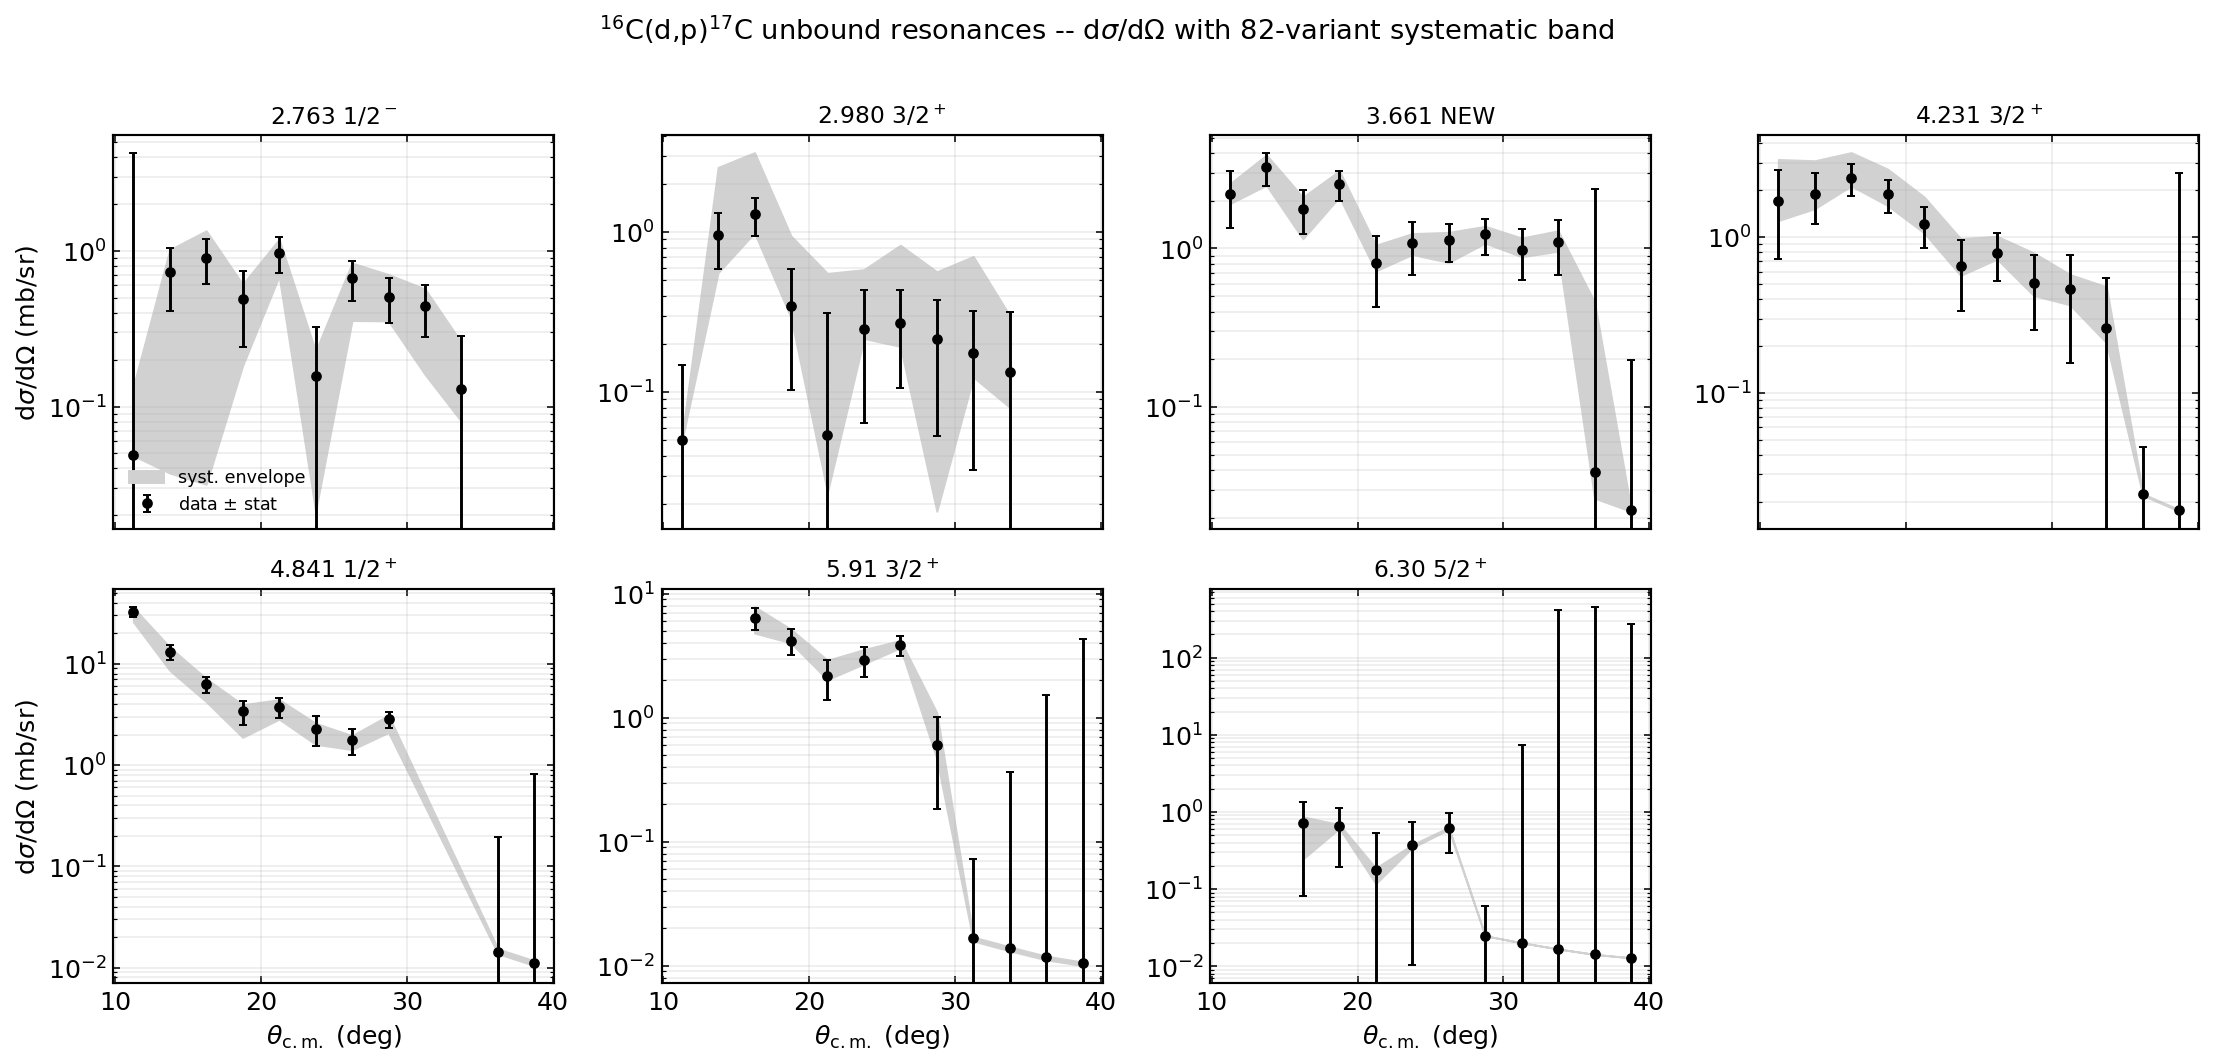
\includegraphics[width=\linewidth]{unbound_ad_grid.png}
  \caption{Angular distributions of the seven unbound \Cse\ resonances. Points:
  data $\pm$ corrected statistical error. Gray band: min--max across the 82
  spectral-fit variants.}
  \label{fig:adgrid}
\end{figure}

\subsection{Method}
Each angular distribution is compared to FRESCO~\cite{Thompson1988} DWBA
single-particle shapes for transferred $L=0,1,2,3$, computed with the
Johnson--Soper ADWA effective deuteron optical
potential~\cite{JohnsonSoper1970} built from the Koning--Delaroche $p+$\Cs\ and
$n+$\Cs\ potentials at $E_d/2$~\cite{KoningDelaroche2003}. All states are
treated in the weakly-bound approximation ($b_e=0.5$~MeV). A single
normalization is fitted per $L$; the best $L$ is the minimum \chinu\ on
\thcm\ $\le30^\circ$. The overlays and the per-$L$ \chinu\ are shown in
Figs.~\ref{fig:fresco} and~\ref{fig:lscan}.

\begin{figure}[t]
  \centering
  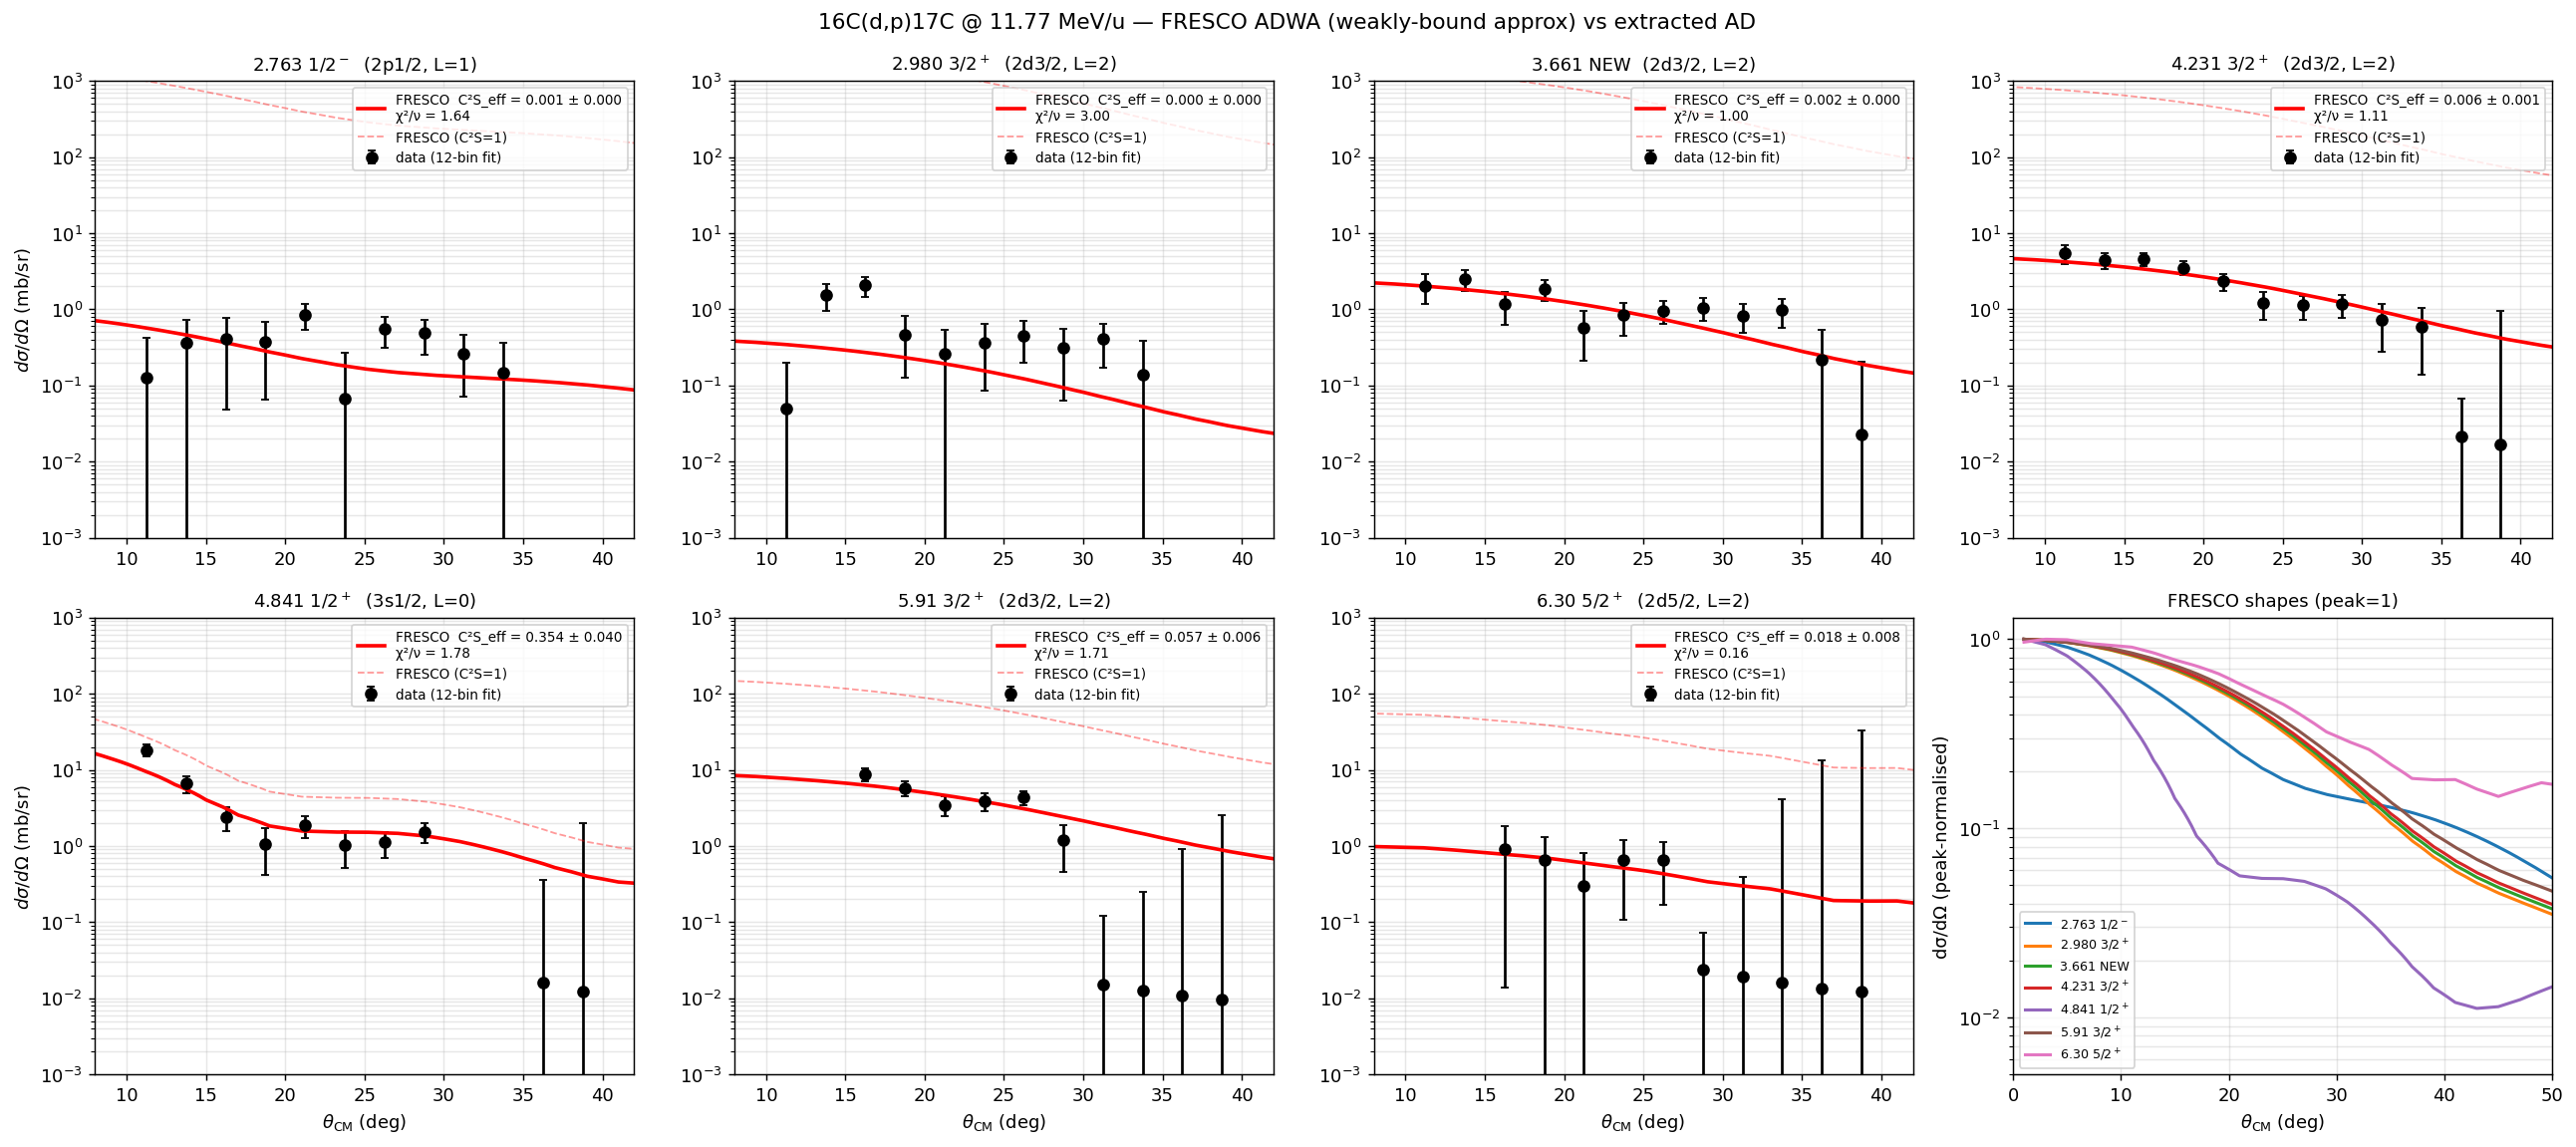
\includegraphics[width=\linewidth]{plots_fresco_unbound.png}
  \caption{Extracted angular distributions (points) with the FRESCO ADWA
  single-particle shape at each state's literature configuration (normalization
  fit over the full $10$--$40^\circ$ range). Note this is distinct from the
  data-driven all-$L$ scan of Fig.~\ref{fig:lscan}, which uses
  \thcm\ $\le30^\circ$.}
  \label{fig:fresco}
\end{figure}

\begin{figure}[t]
  \centering
  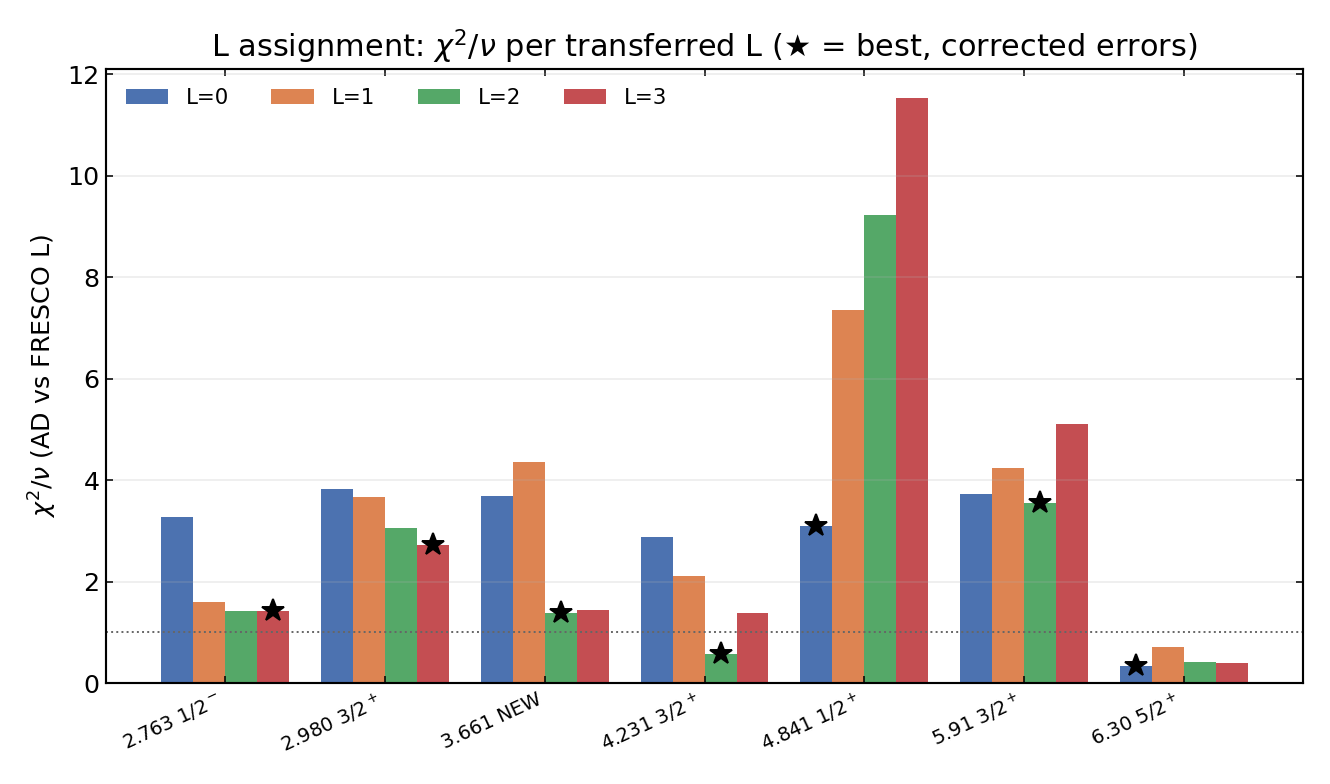
\includegraphics[width=0.72\linewidth]{lscan_bars.png}
  \caption{$\chi^2/\nu$ for each transferred $L$ per unbound state (best $L$
  starred), using the corrected statistical errors.}
  \label{fig:lscan}
\end{figure}

\subsection{Results}
The assignments are summarized in Table~\ref{tab:Lresults}. The \chinu\ values
were refreshed after the per-point error correction; all best-$L$ picks and tie
flags are unchanged, with the absolute \chinu\ rising by a uniform factor
$\sim$$1.3$--$1.5$ (every $L$ scales together).

\begin{table}[t]
  \centering
  \caption{Transferred-$L$ assignments (corrected errors). ``next $L$'' is the
  runner-up; a tie is a runner-up within $0.3$ in \chinu.}
  \label{tab:Lresults}
  \begin{tabular}{cclll}
    \toprule
    $E_x$ (MeV) & lit.\ $J^\pi$ & best $L$ (\chinu) & next $L$ (\chinu) & comment \\
    \midrule
    2.763 & $1/2^-$ & $L{=}3$ (1.41) & $L{=}2$ (1.42) & three-way near-tie; flat AD \\
    2.980 & $3/2^+$ & $L{=}3$ (2.73) & $L{=}2$ (3.05) & all $L$ poor; $17.5^\circ$ peak unfit \\
    3.661 & new     & $L{=}2$ (1.38) & $L{=}3$ (1.45) & $L{=}2/3$ ambiguous \\
    4.231 & $3/2^+$ & $L{=}2$ (0.58) & $L{=}3$ (1.38) & decisive $d$-wave \\
    4.841 & $1/2^+$ & $L{=}0$ (3.09) & $L{=}1$ (7.35) & decisive $s$-wave \\
    5.91  & $3/2^+$ & $L{=}2$ (3.55) & $L{=}0$ (3.73) & $L{=}2/0$ near-tie \\
    6.30  & $5/2^+$ & $L{=}0$ (0.34)$^\dagger$ & $L{=}3$ (0.40) & $\dagger$ $L{=}0$ forbidden; quote $L{=}2/3$ \\
    \bottomrule
  \end{tabular}
\end{table}

Two states warrant caution. For \textbf{2.980}~$3/2^+$ no $L$ template fits well
and the $17.5^\circ$ peak in the angular distribution is not reproduced; the
spectral fit also prefers $E_0$ $\sim$120~keV above the shell-model value. For
\textbf{6.30}~$5/2^+$ the lowest \chinu\ is at $L{=}0$, which is forbidden by the
selection rule $0^+\!\otimes s_{1/2}=1/2^+$; the physically allowed $L{=}2/3$
(essentially tied) should be quoted instead. The final $L$ assignment is
performed downstream by the theory analysis; this work delivers the yields,
\dsdo, and systematic envelope.

\subsection{Effective spectroscopic factors}
The fitted normalizations correspond to effective spectroscopic factors. We do
not present them as a figure here: in the weakly-bound approximation the
single-particle cross section has an artificial, state-dependent magnitude (the
fitted $C^2S_{\rm eff}$ span $\sim$3.5 orders of magnitude), so the angular
\emph{shape} is reliable for $L$ assignment but the \emph{magnitude} is not
physical. Publication-grade spectroscopic factors require a continuum-binned
(CDCC-like) or pole-residue treatment. \note{Insert physical $C^2S$ table/figure
once the CDCC calculation is available.}

% ======================================================================
\section{Non-resonant background and the 0.45~MeV excess}
\label{sec:bg}

\subsection{Is the continuum under control?}
The three non-resonant components (1n phase space, linear background, 2n phase
space) are free in every angular bin, with the phase-space templates rebuilt per
bin. To test their leverage we scaled each component over its full systematic
range ($0.3\times$--$3\times$) and measured the induced fractional change in the
extracted \dsdo\ as a function of angle (Fig.~\ref{fig:bgangle}). The linear
background moves the cross sections by $<2$\,\% (median), flat in angle with no
rise beyond $30^\circ$; the phase-space terms have essentially zero leverage.
The apparent ``onset'' of background near $30^\circ$ is simply the transfer
peaks fading there, not a change in the background itself; the back-angle
limitation is statistics and efficiency, not the continuum.

\begin{figure}[t]
  \centering
  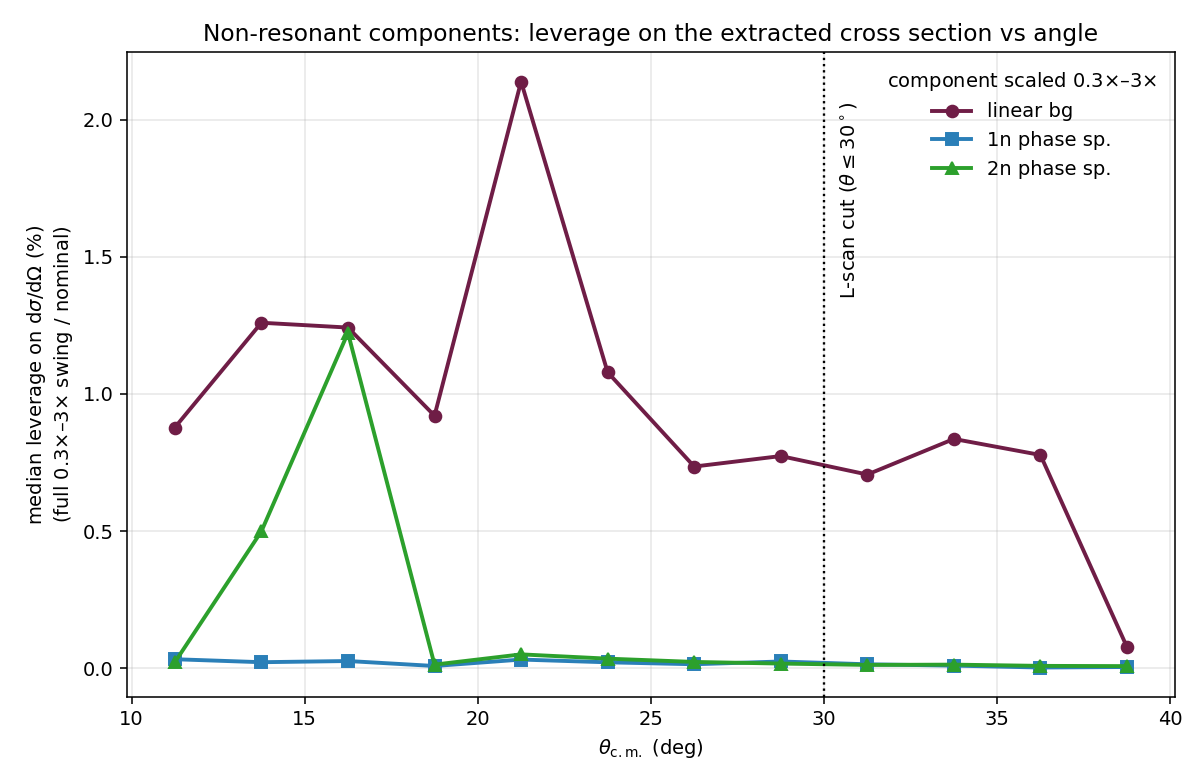
\includegraphics[width=0.7\linewidth]{bg_vs_angle.png}
  \caption{Leverage of the non-resonant components on the extracted \dsdo\ vs
  angle, from scaling each $0.3\times$--$3\times$. The linear background is
  $\lesssim$2\,\% and flat; phase space is negligible.}
  \label{fig:bgangle}
\end{figure}

\subsection{The 0.45~MeV contaminant: angular profile}
The contaminant Gaussian (Sec.~\ref{sec:contam}) is itself a backward-angle
feature: $\sim$87\,\% of its fitted yield lies at \thcm\ $\ge30^\circ$, with the
amplitude pinned near the fit floor at forward angles
(Fig.~\ref{fig:contamangle}).

\begin{figure}[t]
  \centering
  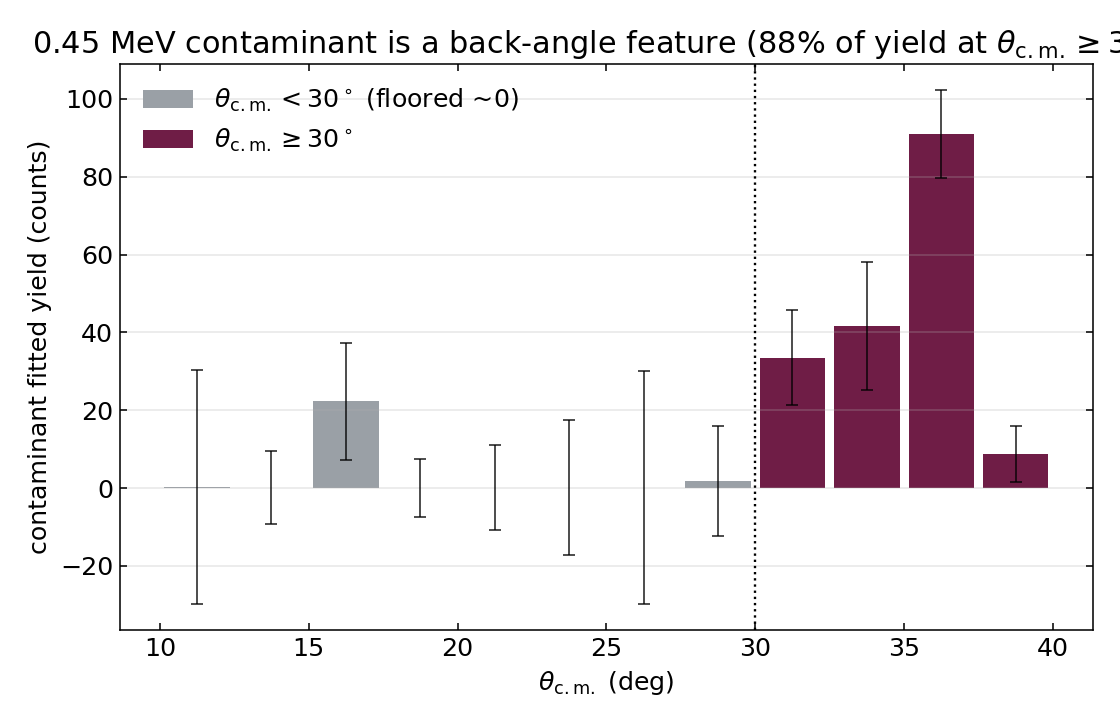
\includegraphics[width=0.62\linewidth]{contam_vs_angle.png}
  \caption{Fitted contaminant yield vs \thcm. The excess concentrates at
  backward angles ($\sim$87\,\% at \thcm\ $\ge30^\circ$).}
  \label{fig:contamangle}
\end{figure}

\subsection{Kinematic fingerprint: inconclusive}
\label{sec:contam-fingerprint}
We attempted to identify the excess as a non-D$_2$ channel by comparing, at
backward angles, the contaminant window ($E_x\in[0.3,1.1]$~MeV) against a
genuine-transfer reference window ($E_x\in[3.5,5.0]$~MeV) in vertex $z$, lab
angle, and proton energy (Fig.~\ref{fig:fingerprint}). This test is
\emph{inconclusive}: the proton-energy comparison is circular, since $E_x$ is
reconstructed from $E_{\rm ej}$ and $\theta$, so any $E_x\simeq0.45$~MeV window
necessarily carries low-$E_x$ kinematics and cannot separate signal from
background. The one $E_x$-independent observable, vertex $z$, shows the
backward-angle contaminant looking like genuine transfer, with no clear spatial
anomaly. The nature of the excess therefore remains open; an $E_x$-independent
discriminant (track quality, spatial clustering, or a slanted-ridge vs vertical-
band test in the $E_x$--$\theta$ plane) is required.

\begin{figure}[t]
  \centering
  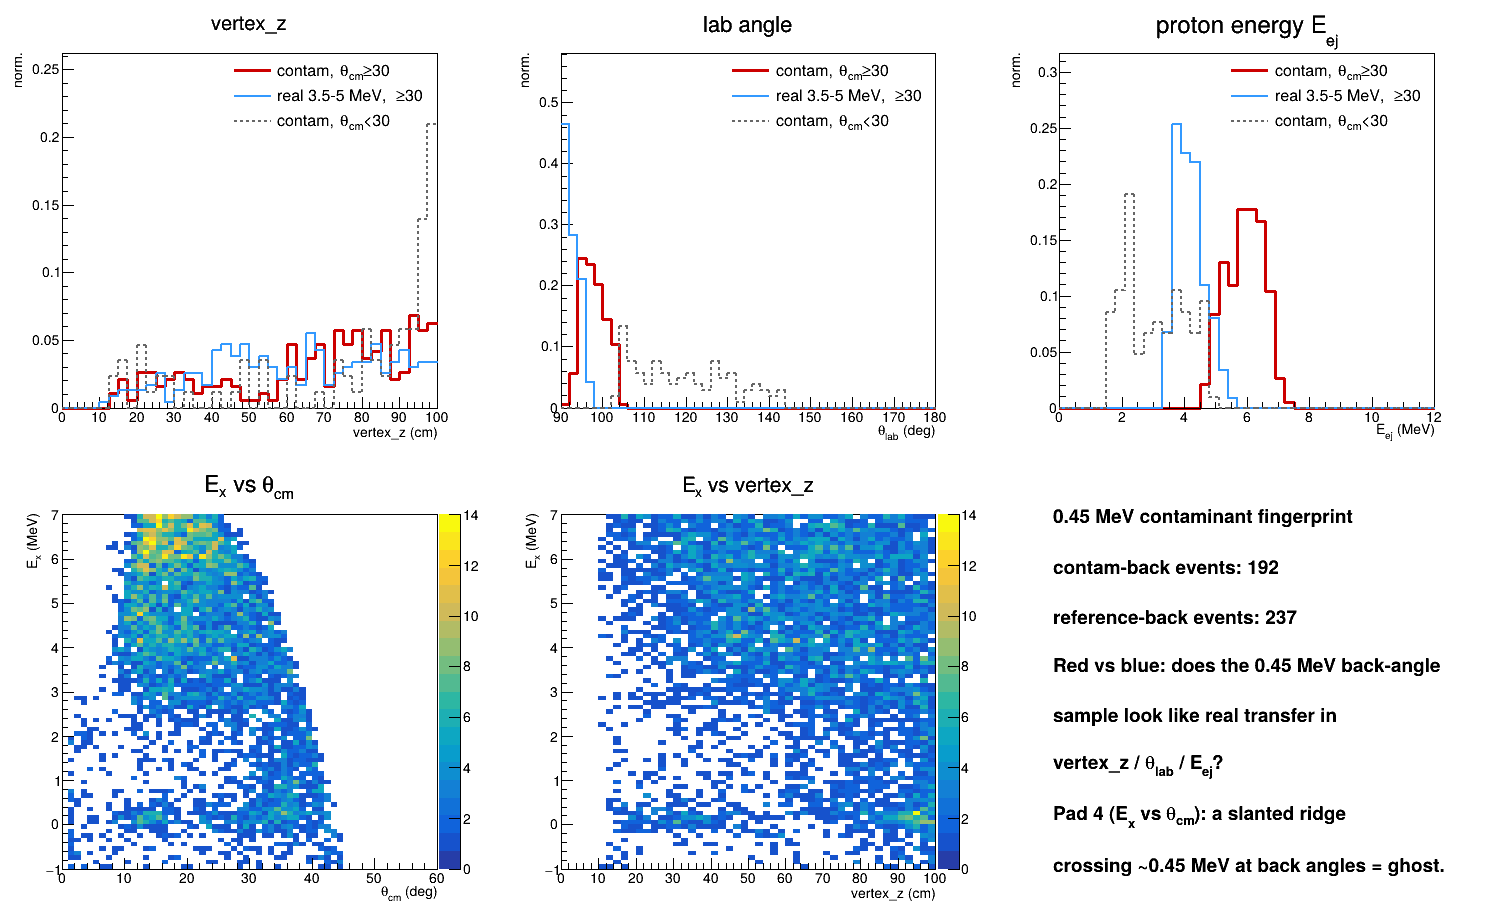
\includegraphics[width=\linewidth]{contam_fingerprint.png}
  \caption{Kinematic fingerprint of the $0.45$~MeV excess (47 runs). Top:
  vertex $z$, lab angle, proton energy for the contaminant window at backward
  angles (red), a genuine-transfer reference (blue), and the contaminant
  forward (gray). Bottom: $E_x$ vs \thcm\ and $E_x$ vs vertex $z$. The test is
  inconclusive (see text).}
  \label{fig:fingerprint}
\end{figure}

% ======================================================================
\section{Systematic uncertainties}
\label{sec:syst}

A campaign of 82 spectral-fit variants spans the model-dependence of the
extraction: BW width scaling ($0.70$--$1.30$), penetrability-$L$ overrides,
state-existence tests, 1n/2n phase-space scaling ($0.3$--$3\times$), linear-
background scaling, the contaminant on/off, relaxed bound-state widths, and the
loose/strict event selection. For each (state, bin) the systematic band is the
min--max of the extracted \dsdo\ across variants
(\texttt{results/systematics\_dsdo\_band\_fine.csv}); the per-state
integrated-yield envelope is shown in Fig.~\ref{fig:yieldenv} and
Table~\ref{tab:yieldenv}.

\begin{figure}[t]
  \centering
  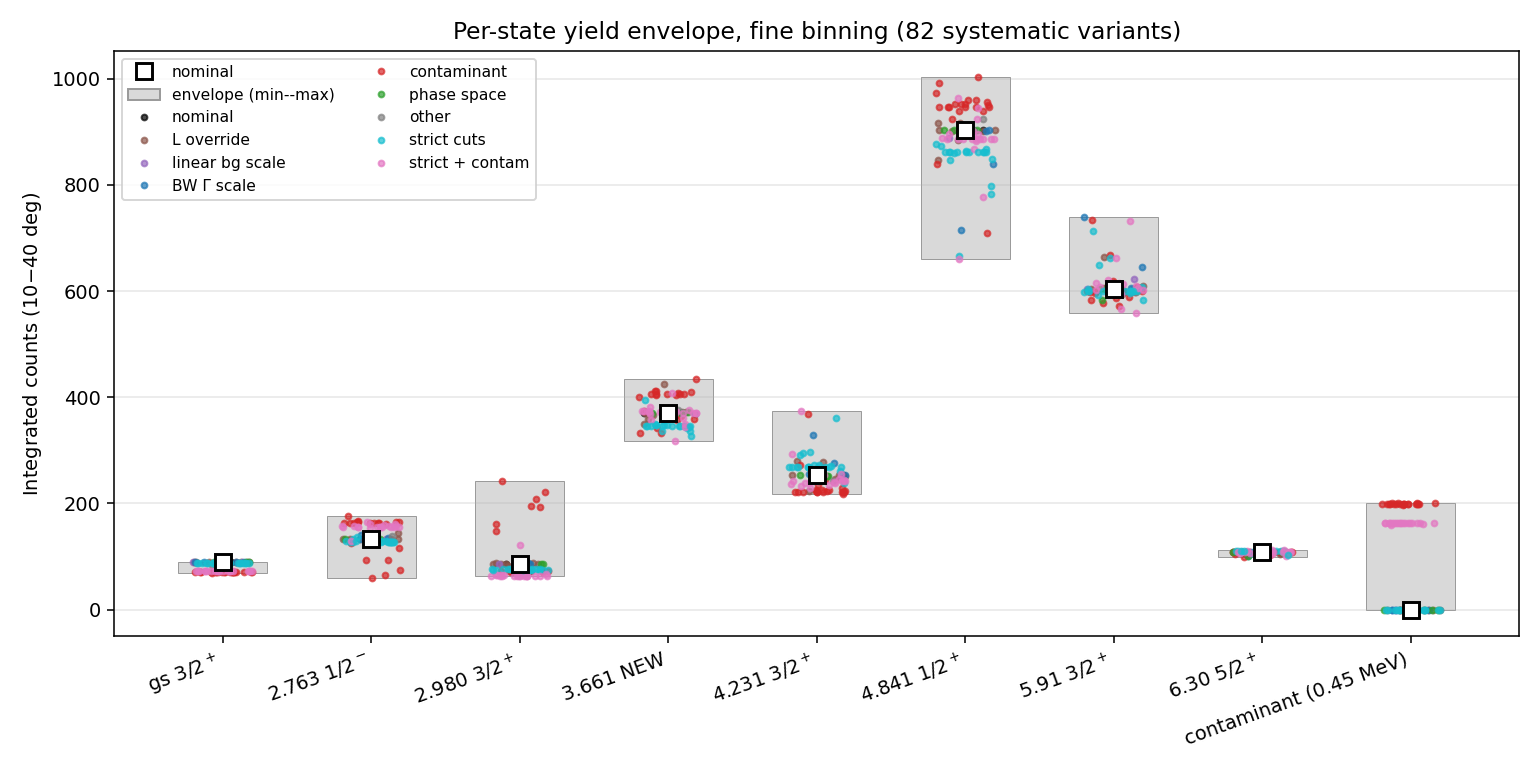
\includegraphics[width=0.7\linewidth]{yield_envelope_fine.png}
  \caption{Per-state integrated-yield systematic envelope (min--max across the
  82 variants).}
  \label{fig:yieldenv}
\end{figure}

\begin{table}[h]
  \centering
  \caption{Per-state integrated-yield systematic envelope (percent deviation
  from nominal).}
  \label{tab:yieldenv}
  \begin{tabular}{lcc}
    \toprule
    state & $-\%$ & $+\%$ \\
    \midrule
    g.s.\ $3/2^+$ & $-23$ & $+0$  \\
    2.763 $1/2^-$ & $-56$ & $+32$ \\
    2.980 $3/2^+$ & $-28$ & $+179$\\
    3.661 new     & $-15$ & $+17$ \\
    4.231 $3/2^+$ & $-14$ & $+48$ \\
    4.841 $1/2^+$ & $-27$ & $+11$ \\
    5.91  $3/2^+$ & $-8$  & $+22$ \\
    6.30  $5/2^+$ & $-9$  & $+3$  \\
    \bottomrule
  \end{tabular}
\end{table}

The picture splits into three groups: \textbf{large} model-dependence for 2.763
and 2.980 (degeneracy with the contaminant); \textbf{moderate} for the higher-
$E_x$ states (driven by the BW width scaling); and \textbf{robust} for 6.30 and
the new 3.661 state. The contaminant-driven uncertainty on 2.980 in particular
should be read as a model-dependence issue, not a statistical one.

The angular-distribution systematic band is shown in
Fig.~\ref{fig:dsdoenv}.

\begin{figure}[t]
  \centering
  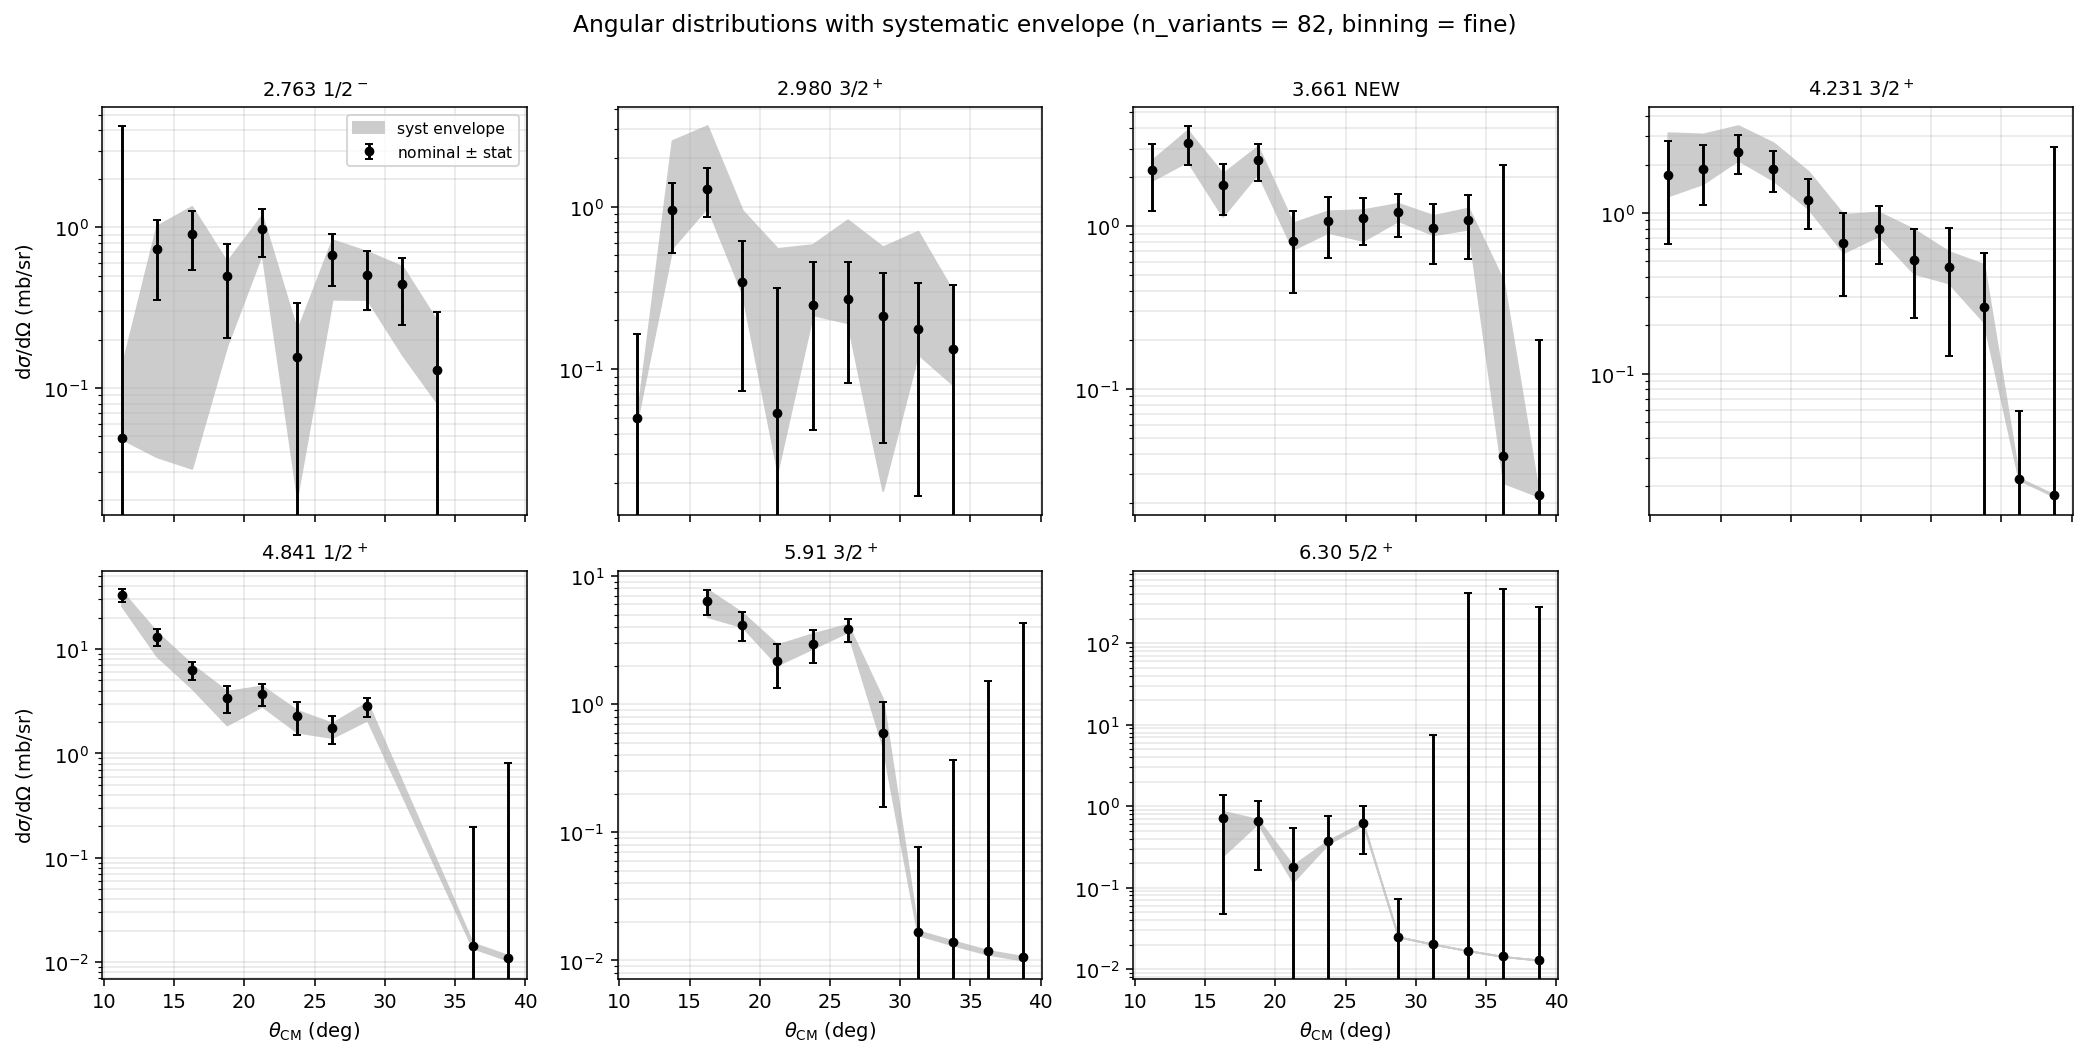
\includegraphics[width=\linewidth]{dsdo_envelope_fine.png}
  \caption{Angular distributions with the 82-variant systematic envelope (gray
  band) overlaid on the nominal points.}
  \label{fig:dsdoenv}
\end{figure}

% ======================================================================
\section{Comparison with previous analyses}
\label{sec:compare}

\subsection{The earlier in-house \Cs\dp\ analysis}
\label{sec:compare-movilla}

The present extraction supersedes, and is benchmarked against, the earlier
\Cs\dp\ analysis of Movilla and Ayyad~\cite{MovillaAyyad2026}, whose reference
fits are reproduced in Figs.~\ref{fig:previnc} and~\ref{fig:prevbin} (copied
verbatim from the parent repository; not regenerated here). The earlier work
used $5^\circ$ angular bins; the present analysis uses $2.5^\circ$ bins, the
$E_x$-dependent efficiency correction, the absolute-normalization validation,
and the corrected per-point error model. The bound-state structure (the three
Gaussians at $0/0.22/0.33$~MeV) and the seven unbound resonances are common to
both; the chief methodological advances here are the absolute scale, the
controlled systematics envelope, and the documentation of the $0.45$~MeV excess.

\begin{figure}[t]
  \centering
  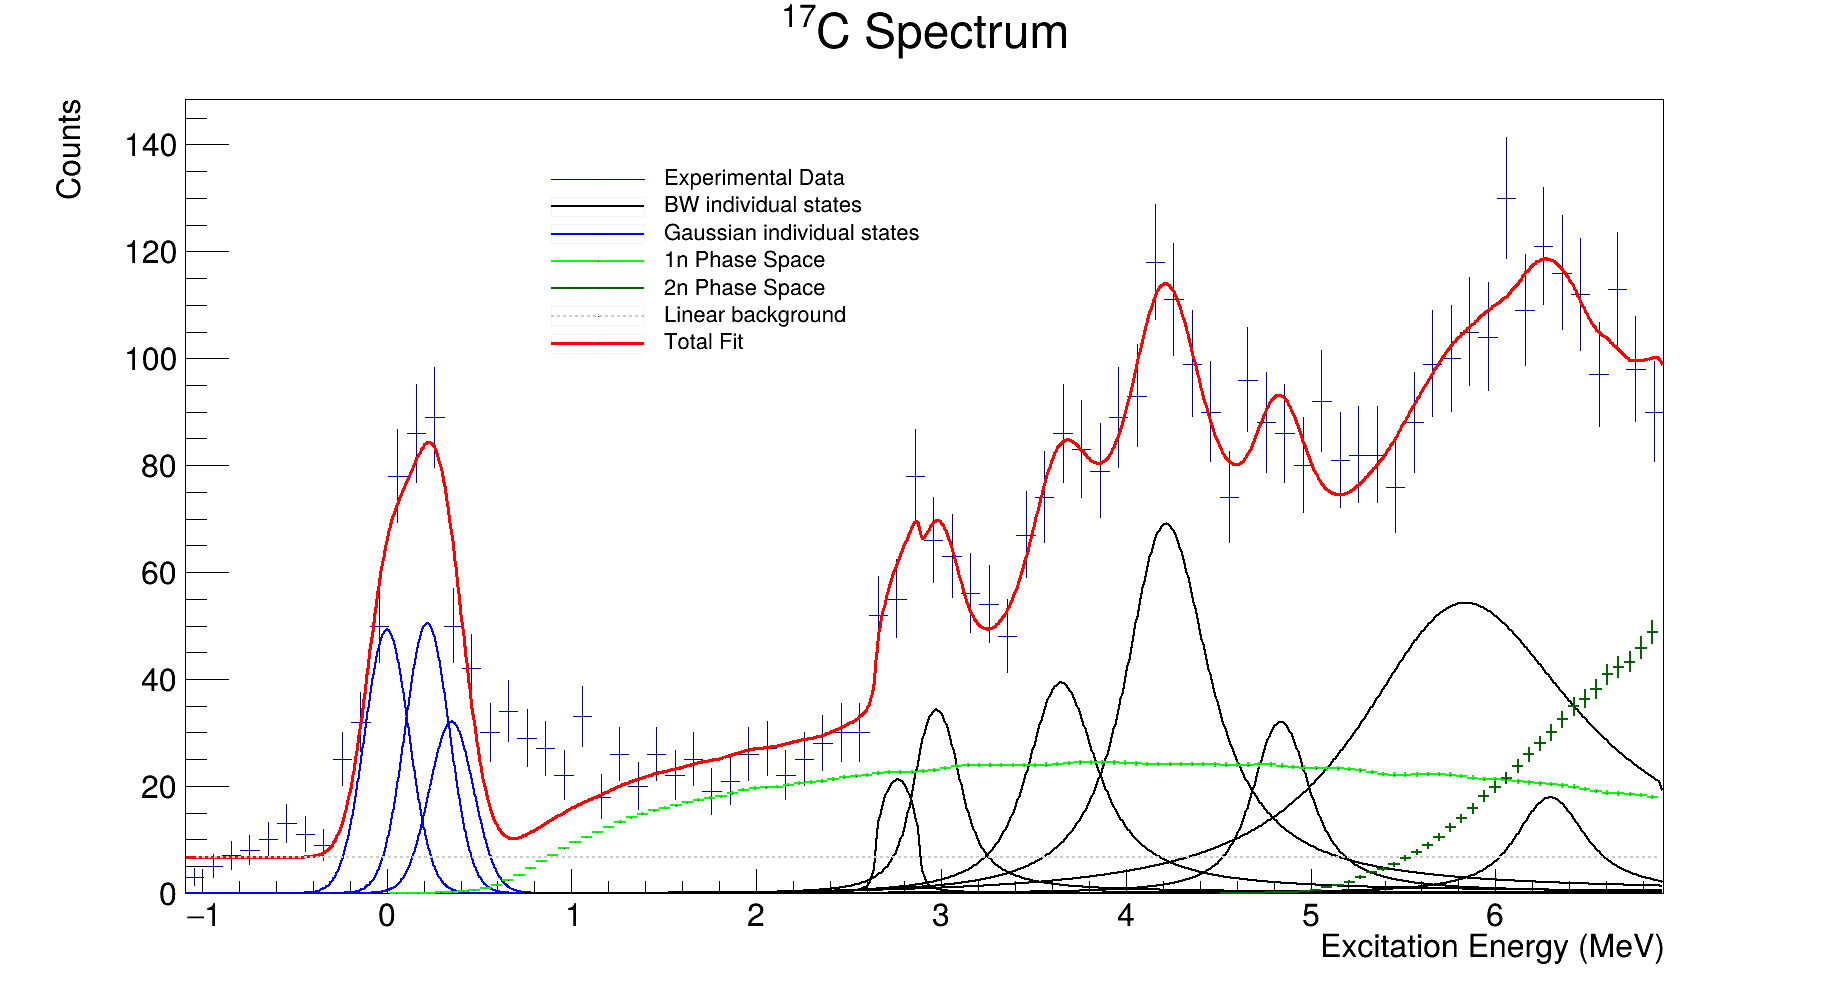
\includegraphics[width=0.72\linewidth]{prev_inclusive.png}
  \caption{Previous-analysis inclusive \Cse\ spectrum (Movilla \& Ayyad). Blue:
  bound-state Gaussians; black: unbound Breit--Wigners; green: phase space.
  Reference only.}
  \label{fig:previnc}
\end{figure}

\begin{figure}[t]
  \centering
  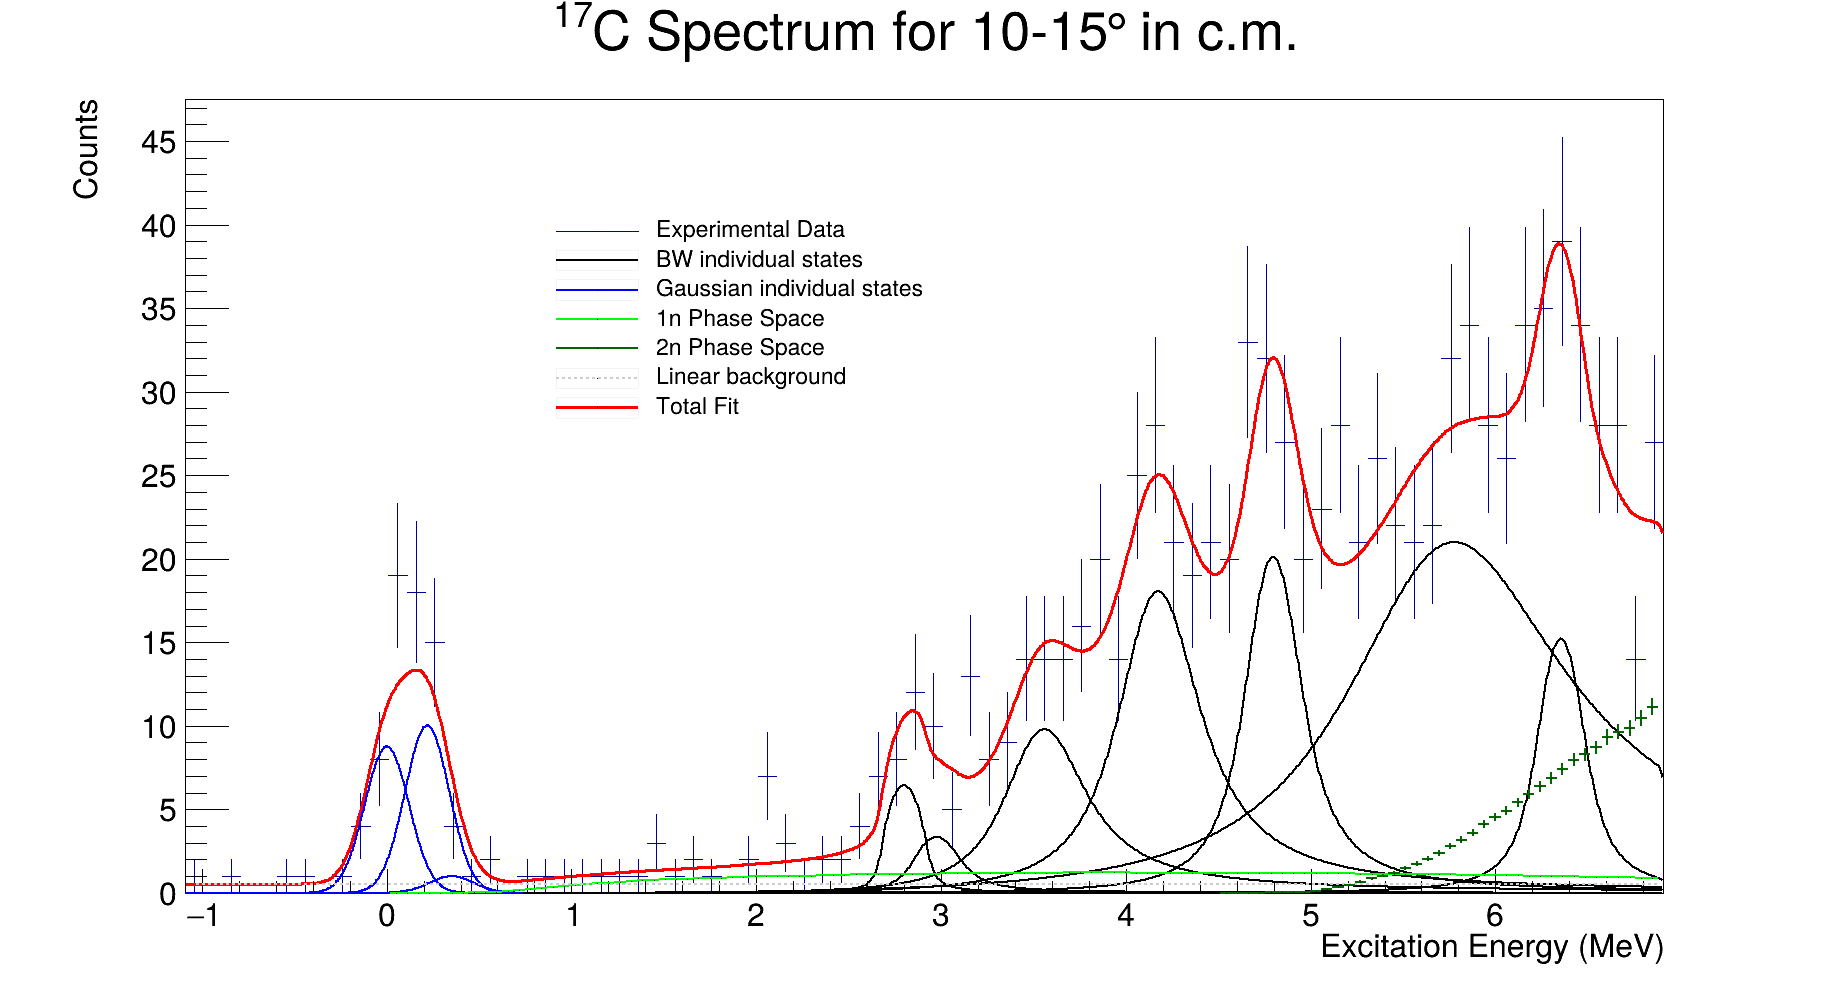
\includegraphics[width=0.72\linewidth]{prev_10-15.png}
  \caption{Example previous-analysis per-bin fit ($10$--$15^\circ$, $5^\circ$
  binning). Reference only.}
  \label{fig:prevbin}
\end{figure}

\subsection{Comparison with Pereira-Lopez \textit{et al.} (PLB 811, 135939)}
\label{sec:compare-plb}

The \emph{bound} states of \Cse\ provide a direct benchmark against the
published transfer measurement of Pereira-Lopez \textit{et al.}, Phys.\ Lett.\
B \textbf{811}, 135939 (2020)~\cite{PereiraLopez2020}, performed at
$17.2$\mevu\ with a finite-range Johnson--Tandy ADWA analysis. This comparison
is carried out in a dedicated companion analysis (repository
\texttt{16Cdp17C\_PLB\_comparison}); the unbound resonances that are the focus
of the present report are not addressed there. We summarize it here for
completeness.

The published angular distributions for the three bound states
(g.s.\ $3/2^+$, $0.217$~MeV $1/2^+$, $0.335$~MeV $5/2^+$), provided directly in
the centre-of-mass frame, are overlaid with the present data on a common
$\theta_{\rm c.m.}$ axis (Fig.~\ref{fig:plboverlay}). FRESCO single-particle
shapes computed at both beam energies ($11.77$ and $17.2$\mevu) and scaled by
the published spectroscopic factors are shown without any additional
normalization. The same data are compared state-by-state against FRESCO
(Fig.~\ref{fig:plbpanels}), and as a coherent sum with the paper's $C^2S$
applied to our DWBA (Fig.~\ref{fig:plbsfs}). The resulting spectroscopic factors
are compared in Table~\ref{tab:plbsf}. The present absolute scale on which this
comparison rests is independently validated against the \Cs$(d,d)$ elastic
channel (Sec.~\ref{sec:norm}), using the same beam$\times$target luminosity
constant.

\begin{table}[h]
  \centering
  \caption{Bound-state spectroscopic factors: Pereira-Lopez \textit{et al.}
  (PLB 811, 135939) versus this work (companion bound-state analysis).}
  \label{tab:plbsf}
  \begin{tabular}{lccc}
    \toprule
    state & $\ell$ & $C^2S$ (PLB) & $C^2S$ (this work) \\
    \midrule
    g.s.\ $3/2^+$   & 2 & $0.03^{+0.05}_{-0.03}$ & $\rightarrow 0$ \\
    $0.217$ $1/2^+$ & 0 & $0.64\pm0.18$          & $\mathbf{0.54\pm0.10}$ \\
    $0.335$ $5/2^+$ & 2 & $0.62\pm0.13$          & $0.47$--$0.74$ \\
    \bottomrule
  \end{tabular}
\end{table}

The $1/2^+$ and $5/2^+$ spectroscopic factors are reproduced within
$\sim$$1\sigma$ using a zero-range Johnson--Soper ADWA on the cleanest
excitation-energy slice. One caveat is documented: at the paper's beam energy
the zero-range calculation misses the deep $\ell=0$ diffraction minimum near
$\theta\simeq17^\circ$, biasing the $1/2^+$ absolute normalization there;
reproducing this requires the finite-range Johnson--Tandy ADWA used in the
published work, which is the natural next step. The bound-state benchmark
nonetheless confirms that the present absolute-normalization and
efficiency-correction chain is consistent with an independent, published
measurement.

\begin{figure}[t]
  \centering
  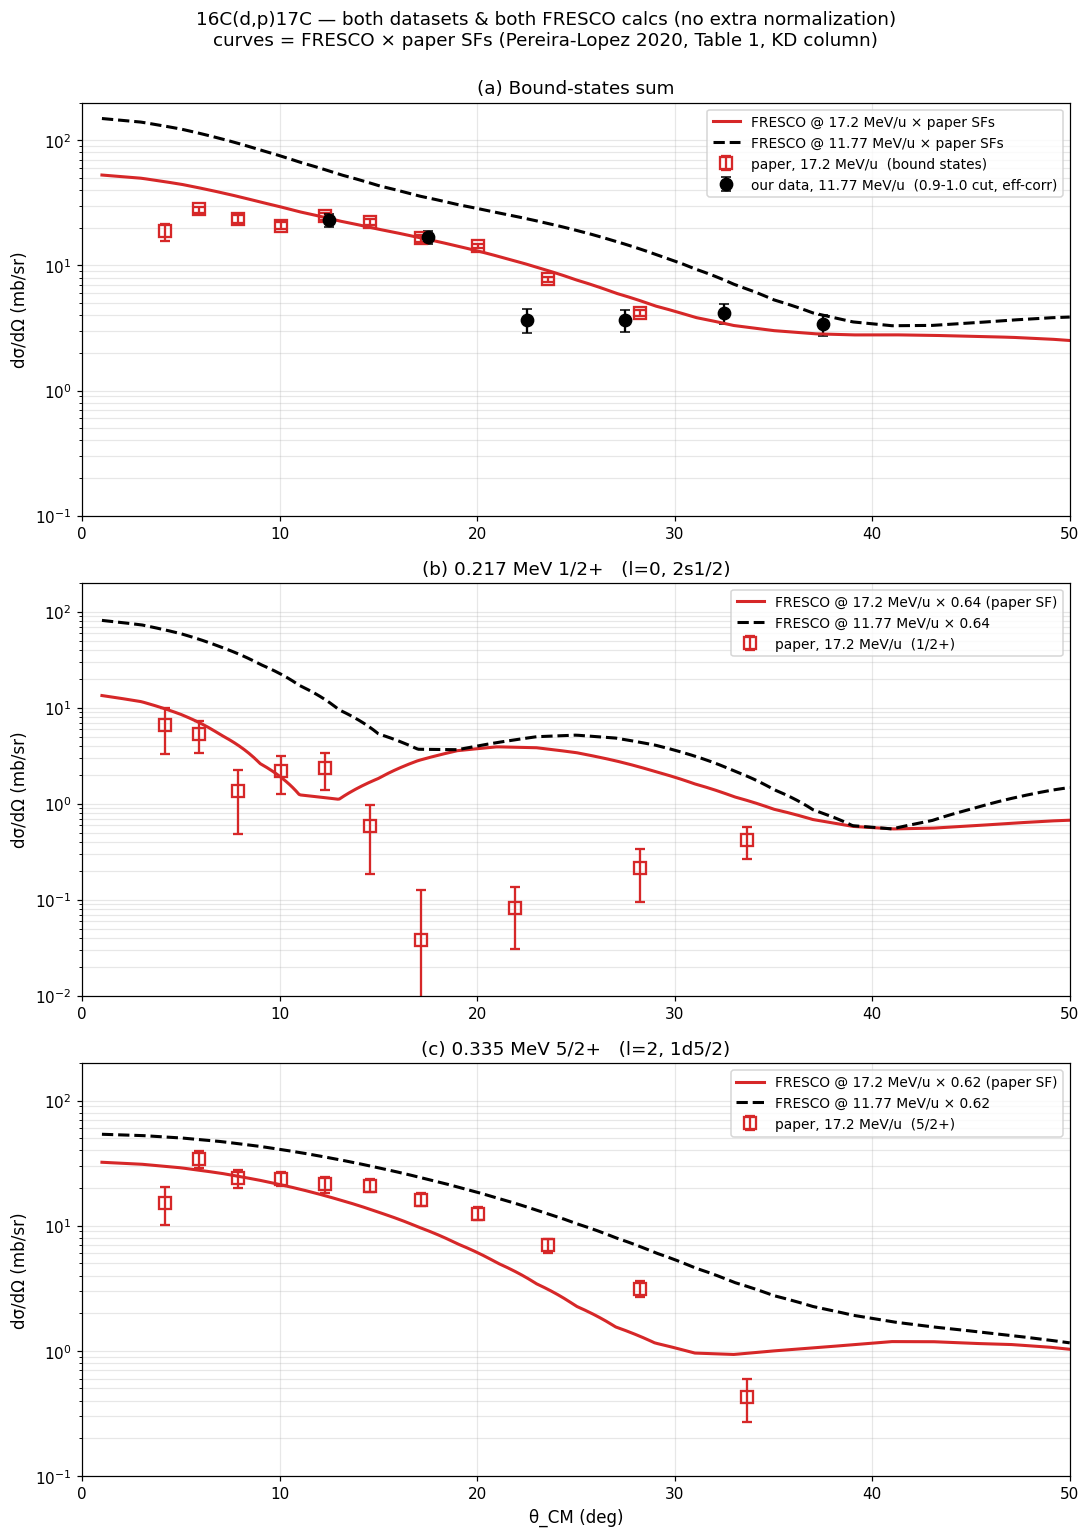
\includegraphics[width=0.62\linewidth]{plb_overlay.png}
  \caption{Bound-state d$\sigma$/d$\Omega$ in the c.m.\ frame, both datasets and
  both FRESCO calculations with no extra normalization:
  (a) bound-states sum, (b) $0.217$~MeV $1/2^+$, (c) $0.335$~MeV $5/2^+$.
  Black: this experiment ($11.77$\mevu); red squares: Pereira-Lopez \textit{et
  al.}\ ($17.2$\mevu, c.m.). Curves are FRESCO at $11.77$\mevu\ (dashed) and
  $17.2$\mevu\ (solid) scaled by the published spectroscopic factors.}
  \label{fig:plboverlay}
\end{figure}

\begin{figure}[t]
  \centering
  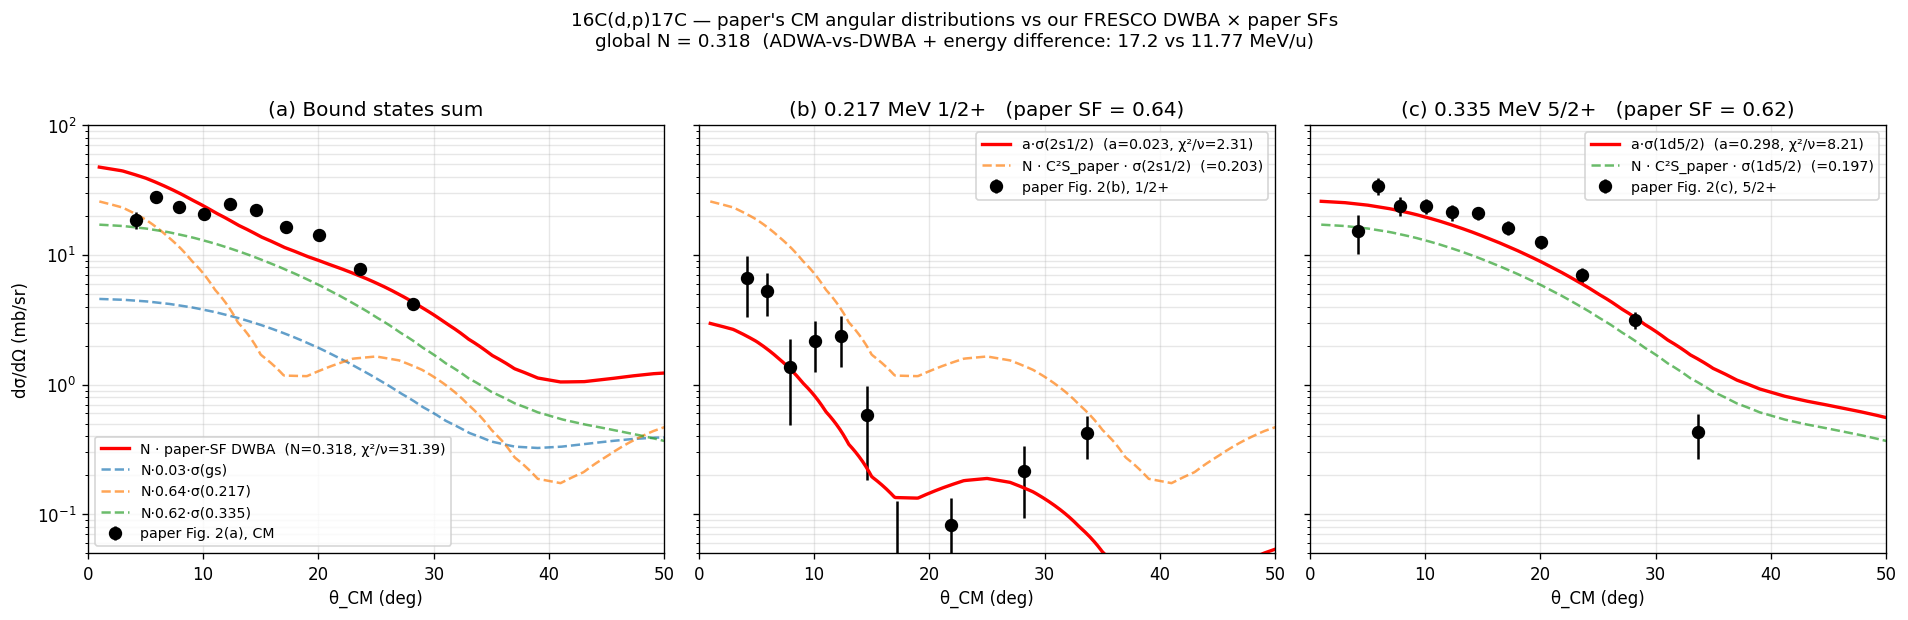
\includegraphics[width=\linewidth]{plb_cm_panels.png}
  \caption{Per-state comparison of the bound-state angular distributions against
  FRESCO with the published spectroscopic factors: (a) bound-states sum,
  (b) $0.217$~MeV $1/2^+$ (paper $SF=0.64$), (c) $0.335$~MeV $5/2^+$ (paper
  $SF=0.62$).}
  \label{fig:plbpanels}
\end{figure}

\begin{figure}[t]
  \centering
  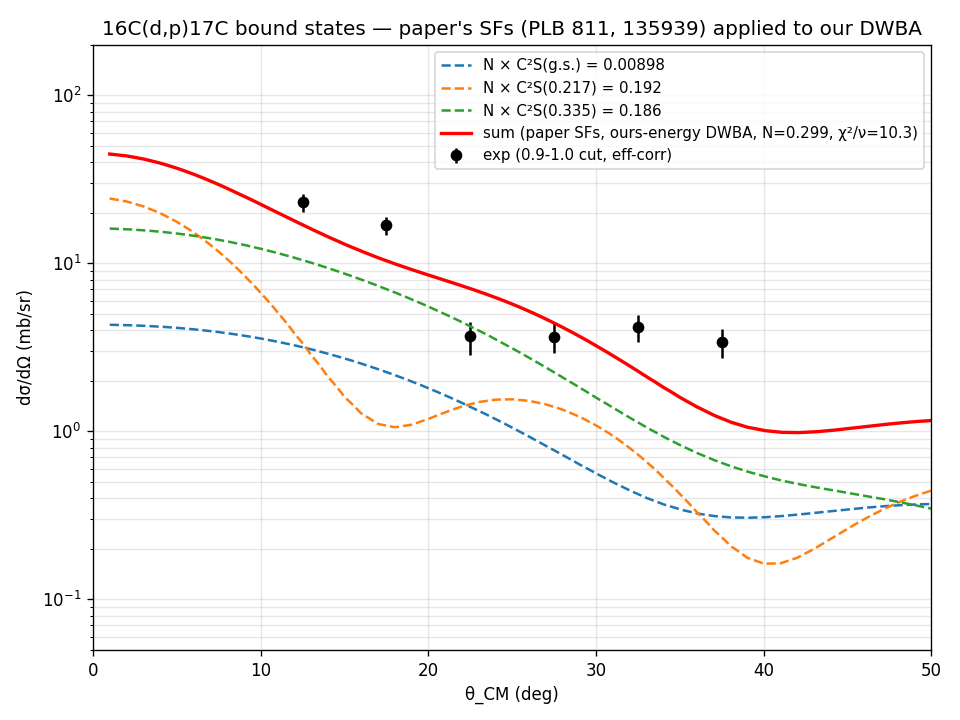
\includegraphics[width=0.72\linewidth]{plb_sfs_overlay.png}
  \caption{Published spectroscopic factors (PLB 811, 135939) applied to our DWBA
  for the three bound states and summed, compared to the efficiency-corrected
  data.}
  \label{fig:plbsfs}
\end{figure}

% ======================================================================
\section{Summary and open items}
\label{sec:summary}

\paragraph{Summary.}
Per-state absolute differential cross sections were extracted for three bound
and seven unbound \Cse\ states from \Cs\dp\ at $11.77$\mevu. The absolute scale
is validated against the \Cs$(d,d)$ elastic channel, with a $\sim$12\,\% global
normalization uncertainty (the optical-potential spread). The per-point error
model was corrected (no double-counting), and statistical, systematic, and scale
uncertainties are kept separate. Transferred-$L$ assignments are robust to the
error correction: $4.231$ ($L{=}2$) and $4.841$ ($L{=}0$) are decisive; $3.661$,
$2.763$, and $5.91$ are ambiguous; $2.980$ and $6.30$ are problematic (shape and
selection-rule respectively). The non-resonant continuum is shown to have
$<2$\,\% leverage on the cross sections, flat in angle. A near-threshold
($0.45$~MeV) excess concentrated at backward angles is documented and carried as
a systematic; a simple kinematic fingerprint was inconclusive.

\paragraph{Open items.}
\begin{enumerate}
  \item \textbf{2.980~$3/2^+$}: resolve the failed $L$ fit (two unresolved
    states? centroid/width? contaminant leakage?).
  \item \textbf{6.30~$5/2^+$}: quote the allowed $L{=}2$, not the forbidden
    $L{=}0$.
  \item \textbf{0.45~MeV excess}: $E_x$-independent discriminants (track
    \texttt{redchisq}, spatial clustering, $E_x(\theta)$ ridge) to settle its
    origin.
  \item \textbf{Absolute $C^2S$}: CDCC / pole-residue treatment for
    publication-grade spectroscopic factors.
  \item \textbf{Normalization scale}: confirm the $\sim$12\,\% correlated band
    is propagated to the final published figures.
\end{enumerate}

\paragraph{Data products.}
All numbers are reproducible from the repository
(\texttt{Yassid/C17\_dp\_fits}): \texttt{results/dsdo.csv} (per-point \dsdo),
\texttt{results/\{dsdo,yield\}\_bands\_fine.csv} (combined bands),
\texttt{results/systematics\_dsdo\_band\_fine.csv} (82-variant envelope),
\texttt{results/fine/L\_scan.csv} ($L$ assignments).

\bibliographystyle{unsrt}
\bibliography{refs}

\end{document}
